\documentclass[a4paper, %draft, 
11pt]{report}

\usepackage[utf8x]{inputenc}
\usepackage[english]{babel}
\usepackage{amssymb}
\usepackage{amsmath}
\usepackage[dvips]{graphicx}
\usepackage{floatflt}
\usepackage{psfrag}
\usepackage{subfigure}
\usepackage{booktabs}
%\usepackage{ctable}
\usepackage{siunitx}
\usepackage[a4paper, centering,margin=1.3in, bindingoffset=0mm]{geometry}
\usepackage{amsmath}
\usepackage{textcomp}
\usepackage[version=3]{mhchem}
\usepackage{multicol}
\usepackage{hyperref}
\usepackage[nameinlink, capitalize]{cleveref}
\usepackage[usenames,dvipsnames]{pstricks}
\usepackage{epsfig}
\usepackage{pst-grad}
\usepackage{pst-plot} % For axes
\usepackage[labelfont=bf, font={small}]{caption}[2004/7/16]
\usepackage{color}
\usepackage{lscape}

\newcommand{\mate}{\begin{equation}}
\newcommand{\atem}{\end{equation}}
\newcommand{\nona}{\nonumber\\&=}
\newcommand{\mai}[1]{\mbox{\footnotesize{\scshape{#1}}}}

\newcommand{\foto}{true}%true=ti conviene che sia true, false=vatti a prendere una pizza finché compila

\title{Photoacoustic observation of \texorpdfstring{\ce{O2}}{} absorption peaks at visible frequencies.}
\author{Zeno Tornasi, Michele Valentini, Henry Widodo}

\begin{document}
	\maketitle
	\tableofcontents
	\chapter*{Introduction}
\addcontentsline{toc}{chapter}{Introduction}

This report presents our final experience for the course of Experimental Physics (advanced), held by prof. M. Scotoni, University of Trento, during academic year 2012/13.

\bigskip
The task was to observe at least one line in the the visible part of the absorption spectrum of \ce{O2} at ambient conditions, using the photoacoustic effect. As a starting point, we have been given a photoacoustic chamber and a red laser diode to excite the oxygen with, together with a case and a controller to adjust the diode temperature and driving current.

\bigskip
In \cref{chapter1} the apparatus and the measurement instruments are globally described, while in \cref{chapter2} we expose some solutions to optimize the apparatus for the measurement we needed to do, as well as some issues we encountered in setting up the most delicate parts.

\medskip
In \cref{chapter3} the collected measurements are presented and discussed. \cref{chamber} deals with the search of the chamber resonance, \cref{oxygen} with the search of the oxygen peaks. \cref{shapeaks} is about the actual observation of the peaks and the study of their shape. \cref{freedrift} contains a small analysis we did on the behaviour of the laser diode. The results in there are important to understand where some effects we encountered across all the previous sections come from.

\medskip
\cref{ECDL,lokkin,etalon} are intended to provide a basic theoretical background about three key elements of our apparatus: the ECDL, the lockin and the etalon.
	\chapter{Description of the apparatus}\label{chapter1}
\section{General overview}
The setup we used featured the typical photoacoustic experiment characteristics. There was a source of light, a laser in our case, impinging on the gas into a cavity. A mechanical chopper provided a modulation of the light in order to match a proper frequency of the cavity. The acoustic signal, detected by microphones, was filtered by a lock-in amplifier referenced with the chopping frequency. The light path was controlled trough optical elements such as mirrors, lenses and beam-splitters (\cref{diagram}).
\begin{figure}[!bhpt]\centering
\includegraphics[width=\linewidth, draft=\foto]{eps/laser_diagram.eps}
\caption{Diagram of the experimental apparatus.}
\label{diagram}
\end{figure}

The laboratory instrumentation shown in \cref{instrument} was used to take measurements and drive the various devices.
\begin{figure}[t]\centering
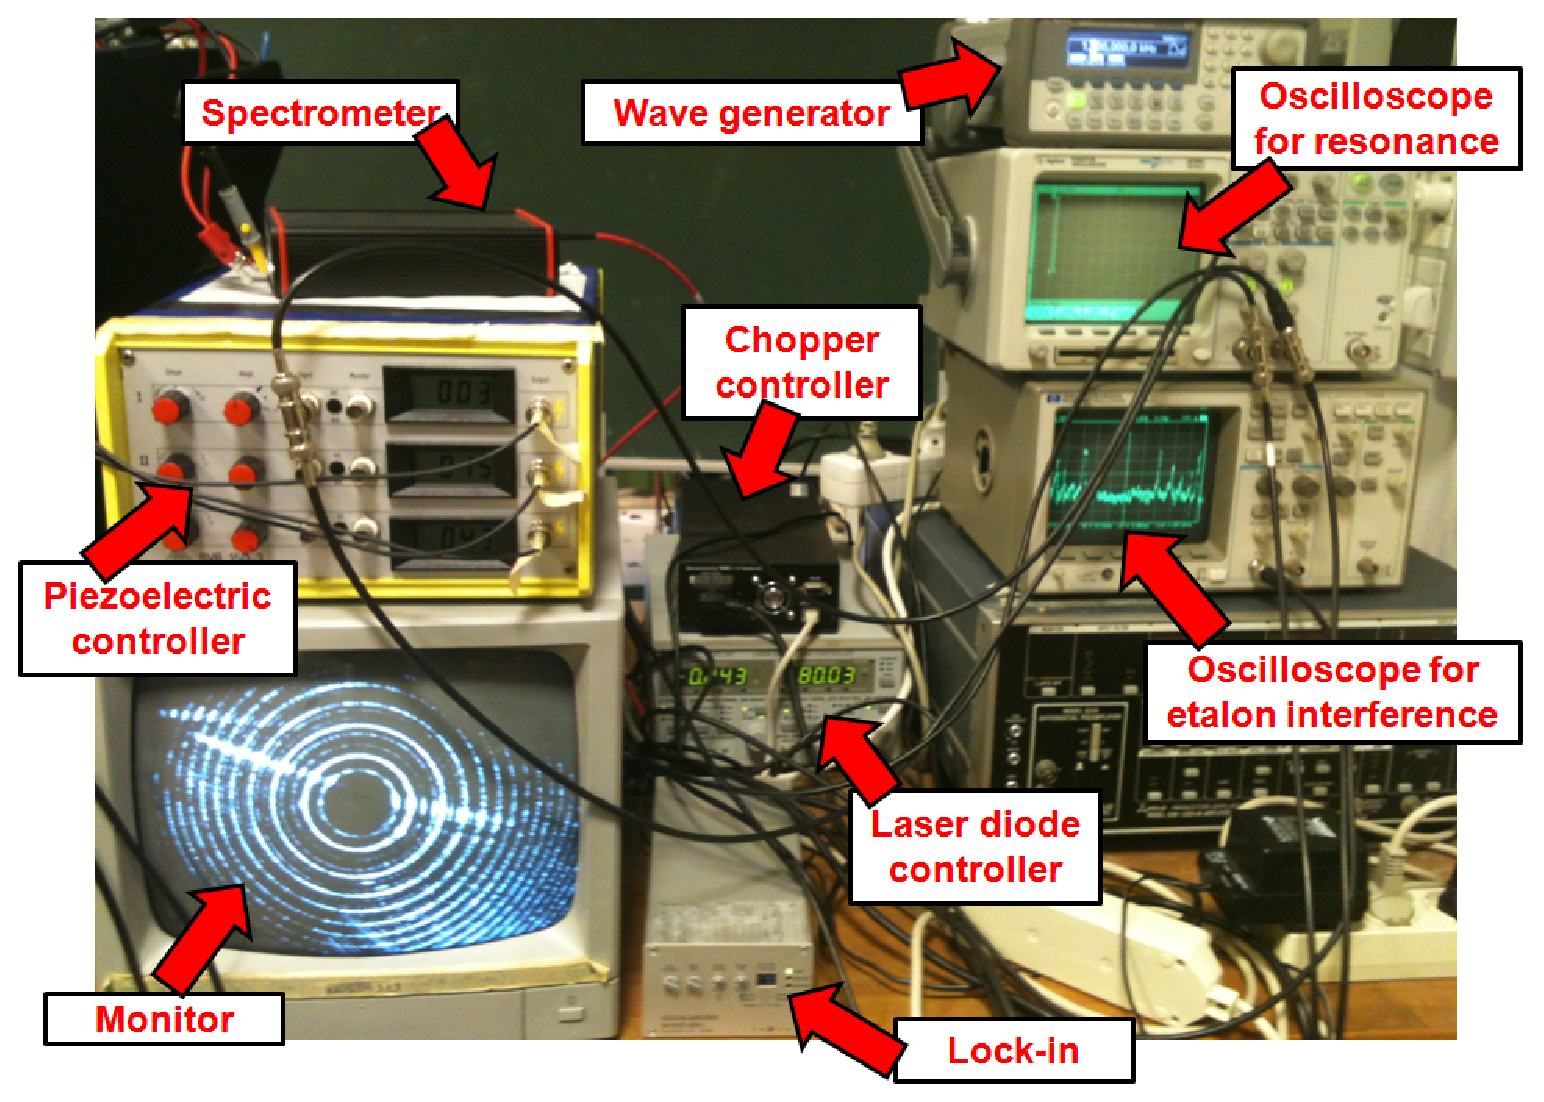
\includegraphics[width=\linewidth, draft=\foto]{eps/instrument.eps}
\caption{Electronic instrumentation used to control the apparatus.}
\label{instrument}
\end{figure}
Other elements we used include:
\begin{itemize}
\item $\pm$15 V power supplier for the microphones
\item membrane vacuum pump
\item rubber pipes and valves to control the gas flow.
\end{itemize}
The data series were acquired with a computer, via a dynamic signal acquisition module\footnote{National Instrument PCI-4462: \url{http://www.ni.com/pdf/manuals/373770j.pdf}}, running the following software:
\begin{itemize}
\item \textit{Avasoft}\textsuperscript{\copyright} by Avantes, the software provided along with the Avaspec spectroscope
\item \textit{Signal Express}\textsuperscript{\texttrademark} by labVIEW\textsuperscript{\texttrademark}
\item \textit{Spectrum}, a labVIEW\textsuperscript{\texttrademark} virtual instrument installed on the laboratory PCs.
\end{itemize}
 We shall now describe in more details the core elements of the apparatus.

 
 \section{Laser source}\label{lasersource}
We used an external cavity laser device, formed by the following elements:
\begin{itemize}
\item a single mode multi-quantum well \ce{AlGaInP}
 laser diode\footnote{Hitachi HL6738MG: \url{http://pdf.datasheetcatalog.com/datasheets/50/502031_DS.pdf}}.
 The lasing wavelength could be tuned from about 680 nm to 695 nm by adjusting the driving current and the diode temperature.
\item a temperature controller case\footnote{Thorlabs TCLDM9: \url{http://www.thorlabs.de/Thorcat/1900/TCLDM9-Manual.pdf}} to set the temperature of the diode. 
\item an external cavity, i.e. a setup that feeds back the laser diode with the first diffraction order of a 1800 grooves/mm grating. Namely, we implemented the so called Littrow configuration (\cref{Littrowsection}). The external cavity allowed us to better select a given lasing mode, thus getting a smaller emission linewidth. The grating was put on a piezoelectric mechanical actuator\footnote{Thorlabs KC1-T-PZ/M: \url{http://www.thorlabs.de/Thorcat/2400/KC1-T-PZ_M-AutoCADPDF.pdf }}, which permitted nm-order adjustments of its position. Since a grating diffracts different frequencies at different angles, moving the grating we could control the frequency fed back to the laser and thus enhanced. This is how we got a fine tuning of the frequency, and how we were able to make the 2-3 GHz scan to see the absorption line (more on this in \cref{tuna}).
\end{itemize} 
\section{Acoustic chamber} 
 The gas to analyze, pure \ce{O2} at atmospheric pressure, was contained in a brass chamber, featuring :
\begin{itemize}
	\item an internal cavity, about \mbox{10 cm} long, where the gas actually resonated. Other two smaller cavities, half as long, were present before and after the main cavity. Since we couldn't open the brass chamber, we had no way to accurately measure the dimensions and the position of the main cavity with respect to the other two ones. It should be noticed that our chamber had been recycled from another experiment and was not explicitly thought for the usage we do of it
	\item four microphones put about halfway in the chamber, one for each side of it. Due to the fact that the chamber couldn't be opened, we don't know whether the microphones were actually halfway. Anyway a possible misplacement would not affect the validity of our measurement, as it would result just in a less intense signal
	\item an active strain gauge vacuometer\footnote{Edwards ASG-1000-NW16:\vspace{-10pt}\begin{flushright}\url{http://www.ultimatevacuum.dk/D35725880\%20ASG\%20user\%20manual.pdf }\end{flushright}} to measure the pressure in the chamber. 
\end{itemize}

\section{Reference arm}\label{referencearm}
Once generated in the ECDL, the laser beam was split by a simple glass into two rays: one going through the chopper and entering the acoustic chamber, the other passing  through an etalon. The interference pattern (see \cref{etalon}) was monitored with a video camera. This was useful, since the the spectroscope resolution, as reported in \cref{tuna}, was too poor to detect the small laser frequency shifts due to fine tuning with the external cavity. The etalon instead could detect this shift as a variation of the diameter in the diffraction rings. Moreover, the PAL analogic video signal could be observed with an oscilloscope as well, to get a quantitative measurement of the rings movements thanks to the measurement functions of the instrument. With respect to the spectroscope, also, the etalon allowed a clearer and faster detection of multi-mode emission 
	\chapter{Experimental setup and hardware improvements} 
Most of our efforts during the experiment were due to the difficulty of finding strong and stable absorption peaks and tuning our laser on such peaks.
The issues encountered during this process can be grouped in these main categories:
\begin{enumerate} 
\item aligning the grating, putting it near the laser in order to minimize the sensitivity to environmental noise sources such as temperature variations and vibrations.
\item focusing the laser beam in the audio cavity without touching the walls.
\item controlling and measuring the laser frequency.
\end{enumerate}
Understanding the behaviour of our apparatus under these aspects was important in order to face the main problem of distinguishing the shape of the absorption peaks from the actually measured peaks, as the latter were distorted by several factors such as mode-hopping and the low-pass filtering of the lock-in amplifier. The subject will be fully discussed in \cref{shapeaks}.

\medskip
The following sections of this chapter will describe how we faced the previously listed experimental challenges.

	\section{Building and optimizing the external cavity laser}
The external laser cavity was described in \cref{lasersource}, while the some theoretical principles about the Littrow configuration ECDL are lined up in \cref{ECDL}. Optimizing this part of apparatus was one of the tasks that required more attention. We ended up in developing the following ideas:
\begin{itemize}
\item We put the grating as near as possible to the laser diode, in order to minimize the sensitivity of the cavity to external factors such as vibrations and cavity length changes due to temperature fluctuations.
\item In order to align as much as possible the first order reflection beam back in the laser, we set the laser current under the original threshold current, i.e. without any external cavity, and adjusted the micrometric screws until we had laser emission at the lower threshold current possible. This procedure also allowed us to obtain the maximum optical power output from the laser. 
\item During the early development of the experimental apparatus the convergent lens included in the LD case was a bit misplaced, so the outgoing beam was not parallel. We didn't know the case could be opened, and we thought we would have had to deal with the beam as it was. Thus we added a small divergent lens between the laser and the grating, in order to make the beam as parallel as possible. This was intended to avoid power losses in the feedback beam and loss of resolution of the grating. (The one-to-one correspondence between angle and diffracted frequency, described in \cref{gratingtheory}, is valid only for a parallel incident wave). Plus we added several other lenses in various points of the apparatus to focus the light and make it parallel. Only later we discovered the possibility of adjusting the position of the first lens (that internal to the case). Fixing that one made unnecessary any other lens in the apparatus.
\end{itemize}

	\section{Focusing the laser in the acoustic chamber}\label{focusing}
The laser beam was not allowed to touch the walls of the chamber, otherwise it would be partially absorbed by them heating up the chamber instead of the gas. This of course could spoil the measurement, generating signal far from the actual absorption wavelength of the oxygen. To avoid this, it was important to perfectly align the beam into the chamber, as well as to make it parallel to avoid a divergence. Moreover, since the beam had not a circular section, we used a slit to cut the sides which could more easily hit the walls. The price was a loss of optical power, of course, but it was worth it to minimize the risk of touching walls.

\medskip

In order to maximize the measured signal we also put a mirror after the chamber which reflected the beam back in the chamber. The alignment of the backwards beam was even more tricky: if we directed it back exactly on the same path of the first beam, it would return into the laser and the whole optical path would act as a second, much longer external cavity. In fact, the two interfered leading to uncontrollable suppression or enhancement of the optical power, as well as driving the laser out of its current lasing mode. To use also the secondary beam, then, it was necessary to align it in such a way that neither did it diverge or touch the walls of the chamber, nor did it collimate with the incoming beam.

	\section{Tuning the laser emission} 
Let's define the \textit{piezoelectric tunability}, to indicate how much we could tune the output frequency of our ECDL by moving the piezoelectric actuators without having the laser to change mode (mode hopping was a serious issue we faced). In order to measure this factor the wavelength resolution of the spectrometer was not sufficient, so we used the etalon combined with the video camera, as described in \cref{referencearm}. Then we made the measurement according to the following procedure:
\begin{enumerate}
\item We measured the distance, in ms of the PAL signal, between the first and the second emission orders (rings) of a mode. This is proportional to the free spectral range of the etalon, as shown in \cref{etalonspec}.
\item We moved the piezoelectric actuators of the maximum amount possible without changing mode, and measured the shift in the position of the first order ring between the two extremal configurations.
\item Comparing this position shift with the FSR, we were able to estimate the piezoelectric tunability.
\end{enumerate}
The estimation we found depended on the laser mode we were trying to tune and ranged from about 2 to 3.5 GHz, with an uncertainty of about 1 GHz estimated from the etalon diffraction peak width.

\medskip
During these measurements we noticed also that the width of the diffraction peaks emitted by the etalon do not correspond to the theoretical 250 MHz calculated from the etalon specifications, but rather to a FWHM of approximately 1-3 GHz (almost the same as the piezoelectric tunability). Several factors could contribute to broaden the width of the peak beyond the original declared performance of the etalon. They are hereafter exposed in order of the importance we assigned to them.
\begin{itemize}
\item The resolution of the camera (the time resolution of the oscilloscope is negligible with respect to the actual width of the ring visualized).
\item The part of the circle we look at (as can be seen by \cref{etalonmonitor} the width of the interference pattern is noisy, thus not perfectly constant around the circle).
\item Dirt and imperfections on the etalon surface.
\item Misalignment and divergence of the impinging beam. An ideal etalon produces zero-width lines only when illuminated by a non-diverging beam.
\item The output bandwidth of the laser, reported in literature to be some tens of MHz, after having been tuned with a ECDL\footnote{L. Ricci et al., \textit{\textquotedblleft A compact grating-stabilized diode laser system for atomic physics\textquotedblright}, Optical Communications 117 (1995) 541-549}.
\item The error in choosing what pixel line to take for the measurement. We could observe only one horizontal line of the screen each measurement. Any pixel line which is not exactly lying on the diameter of the diffraction ring would bring a larger white (illuminated) portion than the actual minimum width.
\end{itemize}
As anticipated before, in controlling the laser emission with the ECDL we faced some big issues with instability and mode hopping. Probably they were due to imperfections in the Littrow configuration ECDL. In principle, the grating should be set in such a way that, by moving the piezoelectric actuators, it only undergoes a rotation without changing the position of the point where the light impinges on it (which actually neither is a point, as a real diode emission has always an extended shape.)

If the aforementioned condition is not fulfilled, that is, if the point where the light hits the grating doesn't lie on the axis of the rotation, then a movement in the actuators causes not only a change in the frequency that is fed back to the laser diode, but also a variation in the length of the external cavity.
	\chapter{Measurements and results}\label{chapter3}
\section{General remarks}
A photoacoustic measurement requires a chopper to modulate the incoming laser at the longitudinal resonance frequency of the chamber, in order to maximize the signal measured by the microphones.

About the microphones, it should be noticed that we didn't know their gain, neither it was possible with our instruments to make a calibration curve. In addition, we thought that understanding in deep the complicated, though interesting, physical processes between the photon absorption and the acoustic wave generation was too far from the general purpose of this work. This implies that, throughout this report, the absorption magnitude signals won't be reported neither with the dimensions of gas absorbance neither with the mechanical dimensions of sound waves. Instead they will be reported in volts, that is, the true (amplified) microphone output that entered the lock-in amplifier. This choice, instead of just using arbitrary units, at least allows us to compare results from different measurements, or even compare our data with those from other groups that used our very same microphones.

\section{Finding chamber resonances}\label{chamber}
The first step of the measurement session was dedicated to find the best resonant frequency. We were told about an approximated length of the internal chamber of 10 cm, hence we expected the first resonating longitudinal mode to be a $\simeq20$ cm long wave. Considering the chamber full of atmospheric pressure \ce{O2} at room temperature, with sound speed 326 m/s this corresponds to a frequency of 1630 Hz.

	\subsection{Open chamber measurement}
We did the measurement stimulating the air inside the chamber through a speaker connected to a waveform generator, and looking at the signal coming from microphones. Since we were not able to insert a speaker inside the chamber (this was small), we excited the open chamber from outside through a hole. The resulting spectrum is shown in \cref{chamberplot}.
\begin{figure}[!t]\centering
% GNUPLOT: LaTeX picture with Postscript
\begingroup
  \makeatletter
  \providecommand\color[2][]{%
    \GenericError{(gnuplot) \space\space\space\@spaces}{%
      Package color not loaded in conjunction with
      terminal option `colourtext'%
    }{See the gnuplot documentation for explanation.%
    }{Either use 'blacktext' in gnuplot or load the package
      color.sty in LaTeX.}%
    \renewcommand\color[2][]{}%
  }%
  \providecommand\includegraphics[2][]{%
    \GenericError{(gnuplot) \space\space\space\@spaces}{%
      Package graphicx or graphics not loaded%
    }{See the gnuplot documentation for explanation.%
    }{The gnuplot epslatex terminal needs graphicx.sty or graphics.sty.}%
    \renewcommand\includegraphics[2][]{}%
  }%
  \providecommand\rotatebox[2]{#2}%
  \@ifundefined{ifGPcolor}{%
    \newif\ifGPcolor
    \GPcolorfalse
  }{}%
  \@ifundefined{ifGPblacktext}{%
    \newif\ifGPblacktext
    \GPblacktexttrue
  }{}%
  % define a \g@addto@macro without @ in the name:
  \let\gplgaddtomacro\g@addto@macro
  % define empty templates for all commands taking text:
  \gdef\gplbacktext{}%
  \gdef\gplfronttext{}%
  \makeatother
  \ifGPblacktext
    % no textcolor at all
    \def\colorrgb#1{}%
    \def\colorgray#1{}%
  \else
    % gray or color?
    \ifGPcolor
      \def\colorrgb#1{\color[rgb]{#1}}%
      \def\colorgray#1{\color[gray]{#1}}%
      \expandafter\def\csname LTw\endcsname{\color{white}}%
      \expandafter\def\csname LTb\endcsname{\color{black}}%
      \expandafter\def\csname LTa\endcsname{\color{black}}%
      \expandafter\def\csname LT0\endcsname{\color[rgb]{1,0,0}}%
      \expandafter\def\csname LT1\endcsname{\color[rgb]{0,1,0}}%
      \expandafter\def\csname LT2\endcsname{\color[rgb]{0,0,1}}%
      \expandafter\def\csname LT3\endcsname{\color[rgb]{1,0,1}}%
      \expandafter\def\csname LT4\endcsname{\color[rgb]{0,1,1}}%
      \expandafter\def\csname LT5\endcsname{\color[rgb]{1,1,0}}%
      \expandafter\def\csname LT6\endcsname{\color[rgb]{0,0,0}}%
      \expandafter\def\csname LT7\endcsname{\color[rgb]{1,0.3,0}}%
      \expandafter\def\csname LT8\endcsname{\color[rgb]{0.5,0.5,0.5}}%
    \else
      % gray
      \def\colorrgb#1{\color{black}}%
      \def\colorgray#1{\color[gray]{#1}}%
      \expandafter\def\csname LTw\endcsname{\color{white}}%
      \expandafter\def\csname LTb\endcsname{\color{black}}%
      \expandafter\def\csname LTa\endcsname{\color{black}}%
      \expandafter\def\csname LT0\endcsname{\color{black}}%
      \expandafter\def\csname LT1\endcsname{\color{black}}%
      \expandafter\def\csname LT2\endcsname{\color{black}}%
      \expandafter\def\csname LT3\endcsname{\color{black}}%
      \expandafter\def\csname LT4\endcsname{\color{black}}%
      \expandafter\def\csname LT5\endcsname{\color{black}}%
      \expandafter\def\csname LT6\endcsname{\color{black}}%
      \expandafter\def\csname LT7\endcsname{\color{black}}%
      \expandafter\def\csname LT8\endcsname{\color{black}}%
    \fi
  \fi
  \setlength{\unitlength}{0.0500bp}%
  \begin{picture}(7200.00,5040.00)%
    \gplgaddtomacro\gplbacktext{%
      \csname LTb\endcsname%
      \put(682,704){\makebox(0,0)[r]{\strut{} 0}}%
      \put(682,1112){\makebox(0,0)[r]{\strut{} 1}}%
      \put(682,1521){\makebox(0,0)[r]{\strut{} 2}}%
      \put(682,1929){\makebox(0,0)[r]{\strut{} 3}}%
      \put(682,2337){\makebox(0,0)[r]{\strut{} 4}}%
      \put(682,2746){\makebox(0,0)[r]{\strut{} 5}}%
      \put(682,3154){\makebox(0,0)[r]{\strut{} 6}}%
      \put(682,3562){\makebox(0,0)[r]{\strut{} 7}}%
      \put(682,3971){\makebox(0,0)[r]{\strut{} 8}}%
      \put(682,4379){\makebox(0,0)[r]{\strut{} 9}}%
      \put(814,484){\makebox(0,0){\strut{} 0}}%
      \put(2012,484){\makebox(0,0){\strut{} 2000}}%
      \put(3210,484){\makebox(0,0){\strut{} 4000}}%
      \put(4407,484){\makebox(0,0){\strut{} 6000}}%
      \put(5605,484){\makebox(0,0){\strut{} 8000}}%
      \put(6803,484){\makebox(0,0){\strut{} 10000}}%
      \put(176,2541){\rotatebox{-270}{\makebox(0,0){\strut{}Magnitude [arbitrary units]}}}%
      \put(3808,154){\makebox(0,0){\strut{}Frequency [Hz]}}%
      \put(3808,4709){\makebox(0,0){\strut{}Open chamber resonances spectrum}}%
      \put(1767,2460){\makebox(0,0){\strut{}1591 Hz}}%
    }%
    \gplgaddtomacro\gplfronttext{%
    }%
    \gplbacktext
    \put(0,0){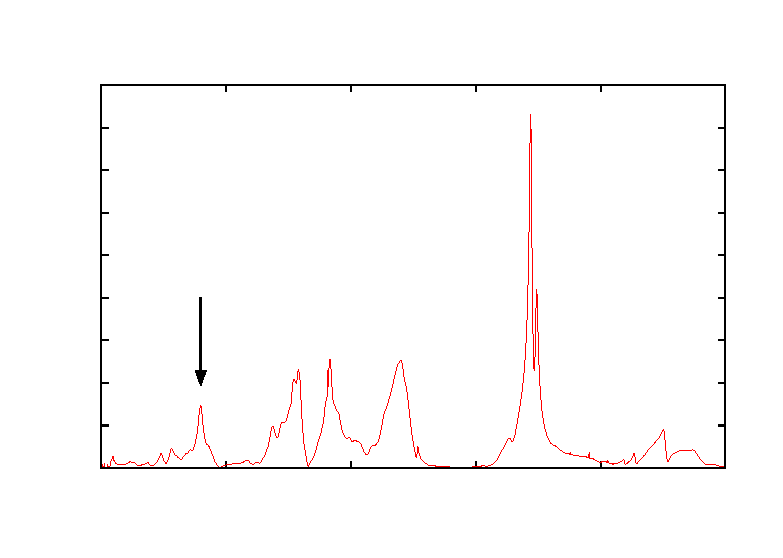
\includegraphics{chamber}}%
    \gplfronttext
  \end{picture}%
\endgroup

\caption{Spectrum of the open chamber, excited with a loudspeaker. The magnitude is set in arbitrary units because this spectrum has been acquired by a software whose unity conversion settings we couldn't control.}
\label{chamberplot}
\end{figure}
In doing this, we differ from the true experimental conditions in three aspects:
\begin{itemize}
\item we have air instead of \ce{O2}
\item we have an open chamber instead of a closed one 
\item the wave signal coming from a small hole aside, instead of being generated in the middle of the chamber.
\end{itemize}

In principle it's easy to correct the spectrum taken in air, in order to apply it to oxygen: in first approximation one has to deal just with a different sound velocity. On the other side, it is more difficult to take into account the acoustic and dynamic modifications the chamber undergoes for being open or closed, as well as for the pressure wave to be originated from a lateral point instead of a diffused volume within the chamber. For these reasons, this cannot be considered as a true spectrum for the chamber we actually used in the absorption measurement. It is nothing more than a useful starting point. Eventually the real resonance frequency had to be experimentally determined with a closed chamber full of oxygen excited from the laser. Also the frequency response of both the loudspeaker and the microphones were unknown, and this could in principle affect the shape of this plot. We looked in a range from 0 to 10 kHz, although we later observed that our chopper wouldn't be able to reach frequencies above few kHz.

We located a clear peak at 1591 Hz, which can attributed to the first longitudinal mode of the chamber, assuming a length $l$ of the chamber slightly greater than the declared 10 cm$$l=\frac{343\mbox{ m/s}}{1591\mbox{ Hz}}\cdot\frac{1}{2}=10.78\mbox{ cm}$$.

		\subsection{Closed chamber measurement}
Starting from the open chamber datum, we injected \ce{O2} in the chamber and began to look for signal by chopping the laser at 1591 Hz. It was promptly clear that there would not be need to further seek for resonances, as the intensity of the signal was high enough even at 1591 Hz, without any correction due to the gas change. We thus decided to delay the search for the acoustic resonance peak in oxygen and proceed with the experiment, in order to save time and give more attention to other issues such as stabilizing the laser emission or look for the oxygen absorption peaks.

Later, at the end of the experiment, we decided that completeness required us to provide the value of maximum resonance with oxygen, even though our measurement were all taken at 1591 Hz. Since the mechanical chopper failed to follow the waveform generator even for the slowest frequency sweep, we couldn't take a spectrum. Changing the frequency by hand we found however the peak at 1512 Hz, where we expected it according to a sound speed in atmospheric pressure oxygen of 323 m/s and a chamber length of 10.78 cm$$f^{\mai{peak}}_{\ce{o2}}=\frac{323\mbox{ m/s}}{2\cdot10.78\mbox{ cm}}\simeq1512\mbox{ Hz.}$$

\section{Looking for the \texorpdfstring{\ce{O2}}{oxygen} peaks}\label{oxygen}
The next step after setting up and optimizing the apparatus was trying to find the best measurement conditions to see the peak. This means to find the frequency of the \ce{O2} absorption peaks, trying the different acoustic resonance frequencies and changing the laser parameters (current, temperature and position of our piezoelectric actuators). 
We were able to measure absorption at various different frequencies, listed in \cref{oxypeaks}:

\begin{table}\centering
\begin{tabular}{|c|}
\hline Wavelength [nm]\\ \hline
686.25 \\ \hline
686.70 \\ \hline
686.75 \\ \hline
686.80 \\ \hline
686.95 \\ \hline
687.05 \\ \hline
687.10 \\ \hline
687.20 \\ \hline
687.25 \\ \hline
687.35 \\ \hline
687.45 \\ \hline
\end{tabular}
\caption{Measured absorption wavelengths for \ce{O2} at ambient pressure and temperature.}
\label{oxypeaks}
\end{table}

During this measurements we first noticed the instability of our laser emission in time. For example, when we found some peak at a certain injection current, temperature and piezoelectric position, after some minutes that peak would drift away and we needed to change the piezoelectric position in order to find it again. After a longer time, like a couple of hours, the peak would decrease in intensity and eventually fade completely, forcing us to change temperature or current of the laser
in order to see it again (or to find some other peak). We are going to discuss more accurately this uncontrolled frequency evolution effect in \cref{freedrift}. 

\section{Shape of the peaks}\label{shapeaks}
\label{factorsinfluencingtheshapeofthepeaks}
After having found some absorption peaks and approximately measured their wavelength using the spectrometer, we tried to acquire their shape as well. As seen in \cref{lasersource}, the piezoelectric tunability was too narrow to acquire one whole peak, so it was important to understand which section of the peak we were looking at. This information allowed us to acquire different points of the same absorption peak, by slightly modifying the output frequency of the laser. The frequency instability in time of the laser output was the biggest deal in doing these measurements. 

As explained in \cref{factorshape}, the shape of the peaks was determined by many parameters. This means that we needed to control all of them (or at least the three most important) at the same time. To do this we used a computer, together with a data acquisition board exploiting four analog inputs, and we were able to log for every single measurement:
\begin{itemize}
	\item the magnitude of the audio wave coming from the lock-in amplifier
	\item the position of the piezoelectric actuator responsible for the rotation of the grating around the $z$ axis
	\item the wavelength of the highest laser peak, measured by the spectroscope software and converted to an analog signal through the integrated DAC
	\item the intensity of such peak or, depending on the needs, the ratio between the intensity of the peak and its integral (in order to detect multi-modal emission).
\end{itemize}

With this setup, the measurements were performed by sweeping the position of the piezoelectric actuators with the waveform generator. We split them in 3 sessions: single full sweeps, multiple full sweeps and multiple focused sweeps.
\subsection{Factors influencing the shape of the peaks}\label{factorshape}
Before discussing the procedures of measuring the shape of the absorption peaks, it was necessary to analyse which factors had influence on this shape in all the measurements we did. The most important ones were mode hopping, multimodal emission and low-pass deformation, which are discussed in the subsequent paragraphs. Other factors such as
\begin{itemize}
\item variations in the speed of the chopper
\item variations in the oxygen pressure and concentration
\item sample rate of our instruments
\item cable capacitance 
\end{itemize}
should have been not relevant when compared to the first three factors.

\subsubsection{Mode hopping} 
Mode hopping is the factor which most distorted the shape of the measured peaks, limiting us to see only a portion of them. As discussed in \cref{tuna}, the linear range of tunability we can exploit to scan the absorption peak is indeed smaller than the peak width. As the laser exits this interval, a mode jump happens, thus making the photoacoustic resonance to fade away. We got around this by logging the wavelength of the emission peak, measured with the spectrometer and calculated by the \textit{Avaspec}\textsuperscript{\copyright} software in real time\footnote{within a response time less than 10$^{-1}$ s.}. Superimposing this data to the acoustic magnitude ones we could distinguish between the parts of the peaks which really corresponded to the absorption peak shape and the parts affected by mode-hopping.

\subsubsection{Multimodes}
The ECDL didn't always emit light on a single wavelength, but often it would emit in 2 or 3, rarely on 4, different wavelengths at the same time. One or more of these emissions could correspond to one of the oxygen absorption lines, thus generating a measurable photoacoustic effect (\cref{multimodes}). This situation rose the problem that the relative intensity of the various emitted wavelengths was not constant even within the tunability range. Therefore the shape of the peak in such situation could be distorted by the change of intensity. In addition, our apparatus could log and register only the wavelength and intensity of the strongest emitted peak, even when the laser was not emitting in a single mode. This made very difficult to distinguish between single-mode and multi-mode emissions just looking at the recorded data. 
Indeed the only way we had to suppose a multi-modal emission according to the recorded data was looking for
\begin{itemize}
\item fast jumps between two wavelengths competing in being the main one
\item decreases in the main peak intensity or in the intensity-peak integral ratio, though difficult because these two parameters were quite noisy.
\end{itemize}
The best solution we found, however, was to personally attend to the measurements and observe the etalon interference pattern to detect multi-modal emissions. Also it was important to try many different sets of laser parameters, in order to avoid multimodal emissions which contained absorption wavelengths.

\begin{figure}
\includegraphics[width=\linewidth, draft=\foto]{eps/multimode.eps}
\caption{We can see two different absorption peaks, both of them appearing during a multimodal laser emission. The first peak corresponds to a wavelength of 687.40 nm but suddenly jumps to a wavelength of 686.65 nm, while the second corresponds to an absorption wavelength of 687.30 nm but jumps back and forth several times between to the frequency of 687.05 nm. This means that the laser is emitting in at least two different modes at the same time and while initially one of the two is the strongest, after a bit the other becomes higher and the spectrometer starts indicating it as the main peak. In such a situation the shape of the peak is severely deformed by the changes in intensity of the various modes.
Laser parameters: 29.10\cel; 73.23 mA.}
\label{multimodes}
\end{figure} 

\subsubsection{Noise and lock-in low pass filter}
The lock-in amplifier we used contained an adjustable low pass filter to control the output signals. A higher time constant allows to filter out more noise, but on the other side it would correspond to a lower slew rate of the signal. This deformed the shape of the peaks, especially when the signal changed abruptly during a mode hop or in fast sweep measurement. After several attempts we found that a time constant of 1 second gave a quite stable output without requiring us to make too slow measurements.
\subsection{Single full sweeps} 
In this kind of measurement, we set the laser diode temperature and injection current, waited about 15 minutes to get emission stability, and started sweeping the piezoelectric crystal along its full driving range (0-150 V), using a linear ramp function with a period of about 11 minutes. This kind of experiment showed all the different absorption peaks available with that choice of laser parameters, and also to study the periodicity of the laser modes with respect to the grating position.

\medskip
\cref{primopicco,moltipicchi} show the result of this first session of measurements. In \cref{fullsweep1} a full sweep of the piezoelectric actuators made the laser to hop its emission mode many times. But only few of those modes met the absorption peak of the oxygen, thus resulting in a high signal. In \cref{fullsweep2} the same modes gives a much lower signal: we moved far away from the absorption peak maximum, even though we didn't change any of the parameters. This is due to the laser frequency drift discussed in \cref{freedrift}.

In \cref{moltipicchi} we slightly changed one of the laser parameters: the diode temperature. The whole modes pattern is now completely reshuffled with respect to \cref{primopicco}, and the full sweep of the piezoelectric actuators shown in \cref{bevified} now highlights three different absorption peaks. A closer observation, in \cref{magnified}, permits to fully appreciate this, as well as to see the signal deformation due to the factors discussed in \cref{factorshape}.
\begin{figure}[!hptb]\centering
\subfigure[Absorption, maximum of a peak. Laser parameters: 29.16 $^\circ$C; 73.23 mA.\label{fullsweep1}]{\includegraphics[width=\linewidth, height=9.5cm, draft=\foto]{eps/660s_first.eps}} 
\subfigure[Absorption, tail of a peak. Laser parameters: 29.16 $^\circ$C; 73.23 mA.\label{fullsweep2}]{\includegraphics[width=\linewidth, height=9.5cm, draft=\foto]{eps/660s_second.eps}}
\caption{Photoacoustic absorption of a $\simeq$ 687.0 nm peak. The wavelength shift between the two plots is of the order of $10^{-2}$ nm, thus it's not visible on the scale. The noisy parts at $\simeq220$ s are due to the fast backwards ramp of the sweeping.}\label{primopicco}
\end{figure}

\begin{figure}[!hptb]\centering
\subfigure[Laser parameters: 29.06 $^\circ$C; 73.23 mA.\label{bevified}]{\includegraphics[width=\linewidth, height=9.5cm, draft=\foto]{eps/660s_third_normal.eps}} 
\subfigure[Magnification of the previous plot.\label{magnified}]{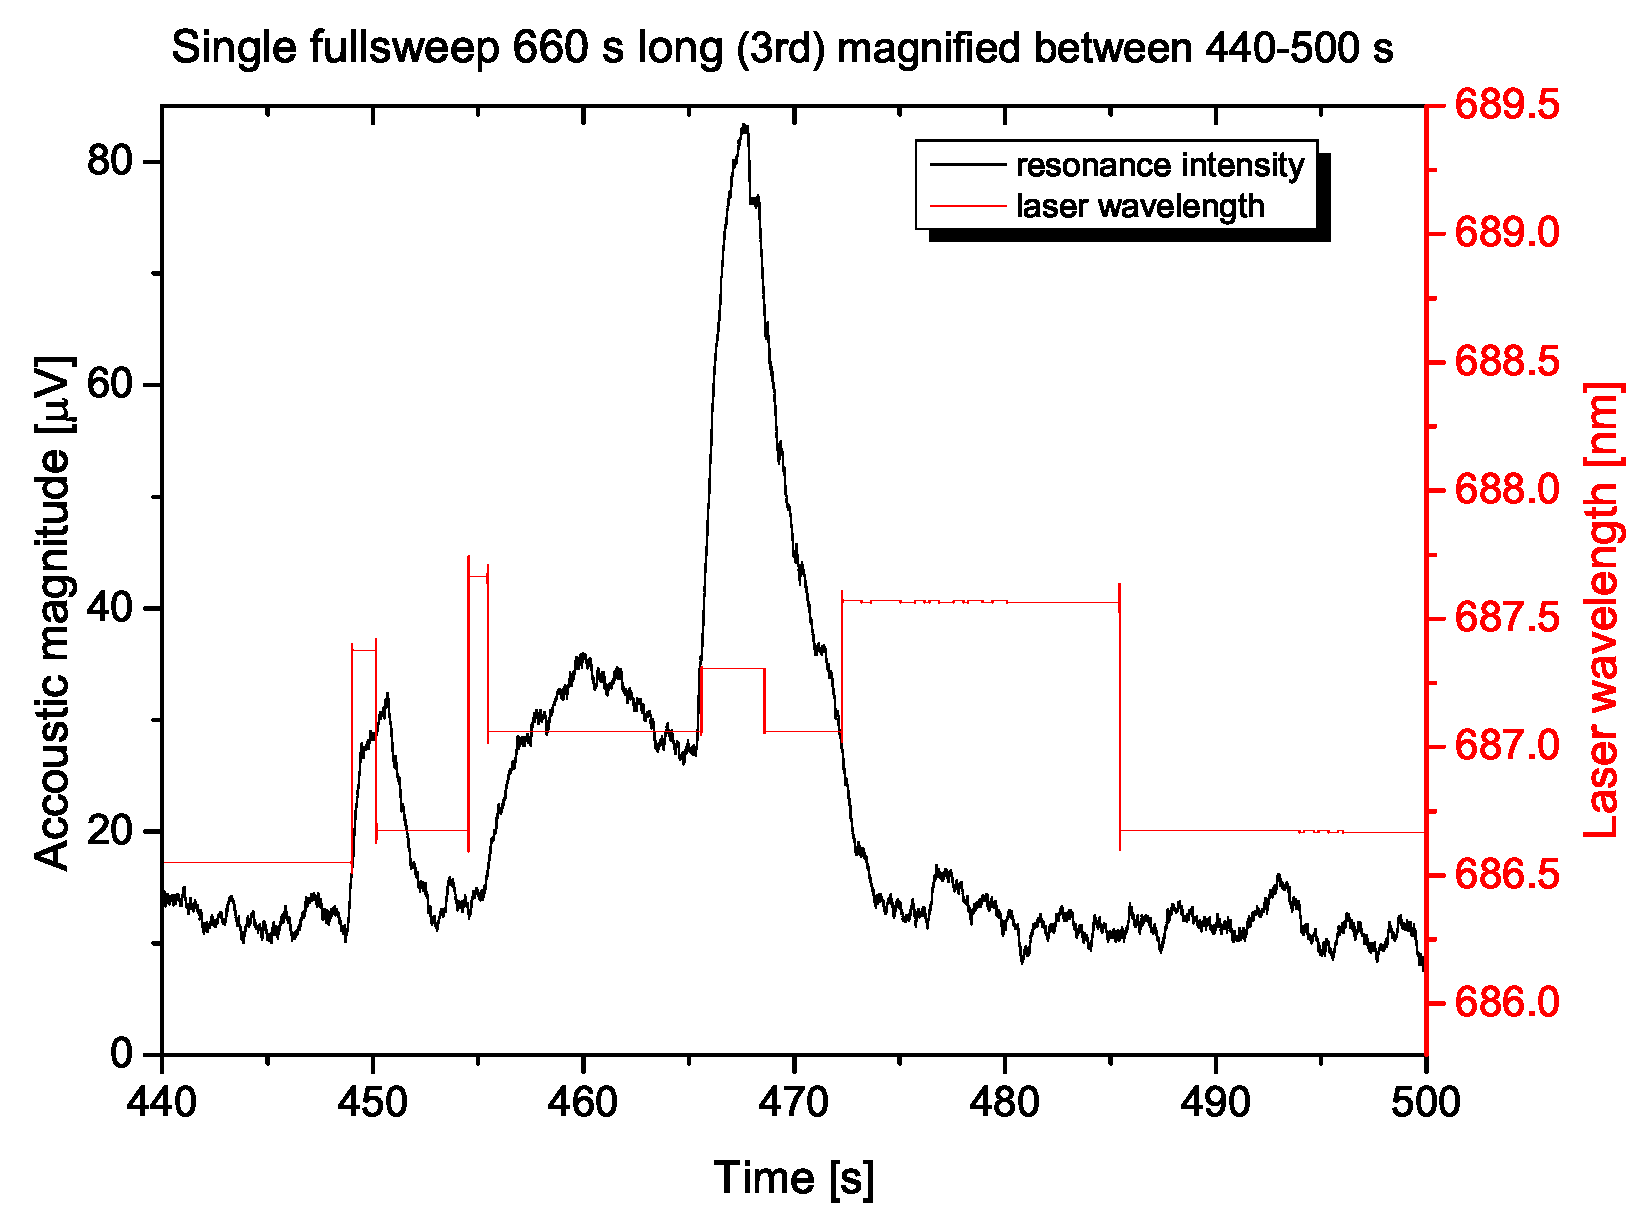
\includegraphics[width=\linewidth, height=9.5cm, draft=\foto]{eps/660s_third_magni.eps}}
\caption{In this measurement, the laser diode temperature is 0.1 $^\circ$C lower than \cref{primopicco}. We notice 3 different absorption wavelengths: 687.30, 687.35, 687.05 nm. Here are visible the deformations we studied in \cref{factorshape}}\label{moltipicchi}
\end{figure} 

\medskip
Looking at the peak wavelength plots we noticed that the laser mode jumping is somehow periodical with respect to the piezoelectric sweeping voltage. That is, for portions of the sweep about 50-100 V large the modes hop from one to another according to a constant pattern.
This can be easily seen in \cref{hoppattern}, which shows both the wavelength of the main emission peak and its intensity, during part of the sweep shown in \cref{fullsweep1}. The pattern, followed clearly for at least a couple of periods, is shown in \cref{tabrutta}.

\begin{figure}[!hbpt]\centering
\includegraphics[width=\linewidth, height=10cm, draft=\foto]{eps/periodicityofhops.eps}
\caption{We can see that the laser follows the same hopping pattern for several seconds, corresponding to a piezoelectric voltage sweep of 75 V.}
\label{hoppattern}
\end{figure}

\begin{table}[!hbpt]\centering
	\begin{tabular}{|c|c|}
	\hline	Time interval [s]&Wavelength [nm]\\
		\hline
0&687.45\\ \hline%339
5&686.60\\ \hline
21&687.40\\ \hline
24&687.65\\ \hline
27&687.05\\ \hline
39&687.30\\ \hline
39&687.05\\ \hline
41&687.55\\ \hline
55&686.95\\ \hline
	\end{tabular}
\caption{Example of hopping pattern. The time intervals are calculated from the beginning of \cref{hoppattern}, 339 s.}
\label{tabrutta}
\end{table}

%DA QUI A QUI STAVA QUI
% (scrivere di come in effetti sto aumento virtuale non sia quasi mai stato possibile da misurare a causa deella deformaz dei picchi dovuti alle instabilità o al semplice fatto che la nuova parte visibile è irrilevante (non contiene picco). 

	\subsection{Multiple full sweeps}
Since these measurement took quite a long time every sweep, doing repeated measurements most of time resulted in unmatchable data, because of the uncontrolled evolution we already mentioned. The influence of such uncontrolled factors exhibited however a random behaviour, so that, after some trials, we were able to get a unique \textquotedblleft lucky\textquotedblright measurement of 3 subsequent sweeps which matched almost perfectly. This is shown in \cref{3sweep}.

All the other attempts, instead, resulted in severe changes of the resonance pattern between one sweep and another. Studying the pattern of the wavelength vs voltage graphic helps in realizing that this difference is not to be ascribed to the photoacoustic part of the experiment (oxygen concentration/pressure, laser alignment) but is rather due to a change in the laser emission wavelength pattern. \cref{3missweep,7sweeps} provide meaningful examples of this behaviour.
The change in the wavelength pattern is better shown in \cref{focus}, where we focused
on shorter multiple sweeps around a single absorption peak.
\begin{landscape}
\begin{figure}[!bhtp]\centering
\includegraphics[height=\textheight, draft=\foto]{eps/3sweepsmatching.eps}
\caption{Three subsequent 0-150 V sweeps, of duration of 11 minutes each. Red: acoustic signal magnitude vs time and actuators voltage. Green: time projection. Blue: voltage projection. Notice that in the voltage projection the matching between the peaks of different sweeps in almost perfect. Laser parameters: 29,50 $^\circ$C; 80,01 mA.}
\label{3sweep}
\end{figure}\vfill
\end{landscape}

\begin{landscape}
\begin{figure}[!bhtp]\centering
\includegraphics[height=\textheight, draft=\foto]{eps/3mismatching.eps}
\caption{Despite these measurements are taken faster then usual (5 minutes each 0-150 V sweep) there is a big mismatch between the three sweeps. This mismatch is more evident in the magnitude vs voltage projection, where the peaks seem to be double-peaks. The time projections shows instead that they are
single peaks. Laser parameters: 27,68\cel; 80,01 mA}
\label{3missweep}
\end{figure}\vfill
\end{landscape}

\begin{landscape}
\begin{figure}[!bhtp]\centering
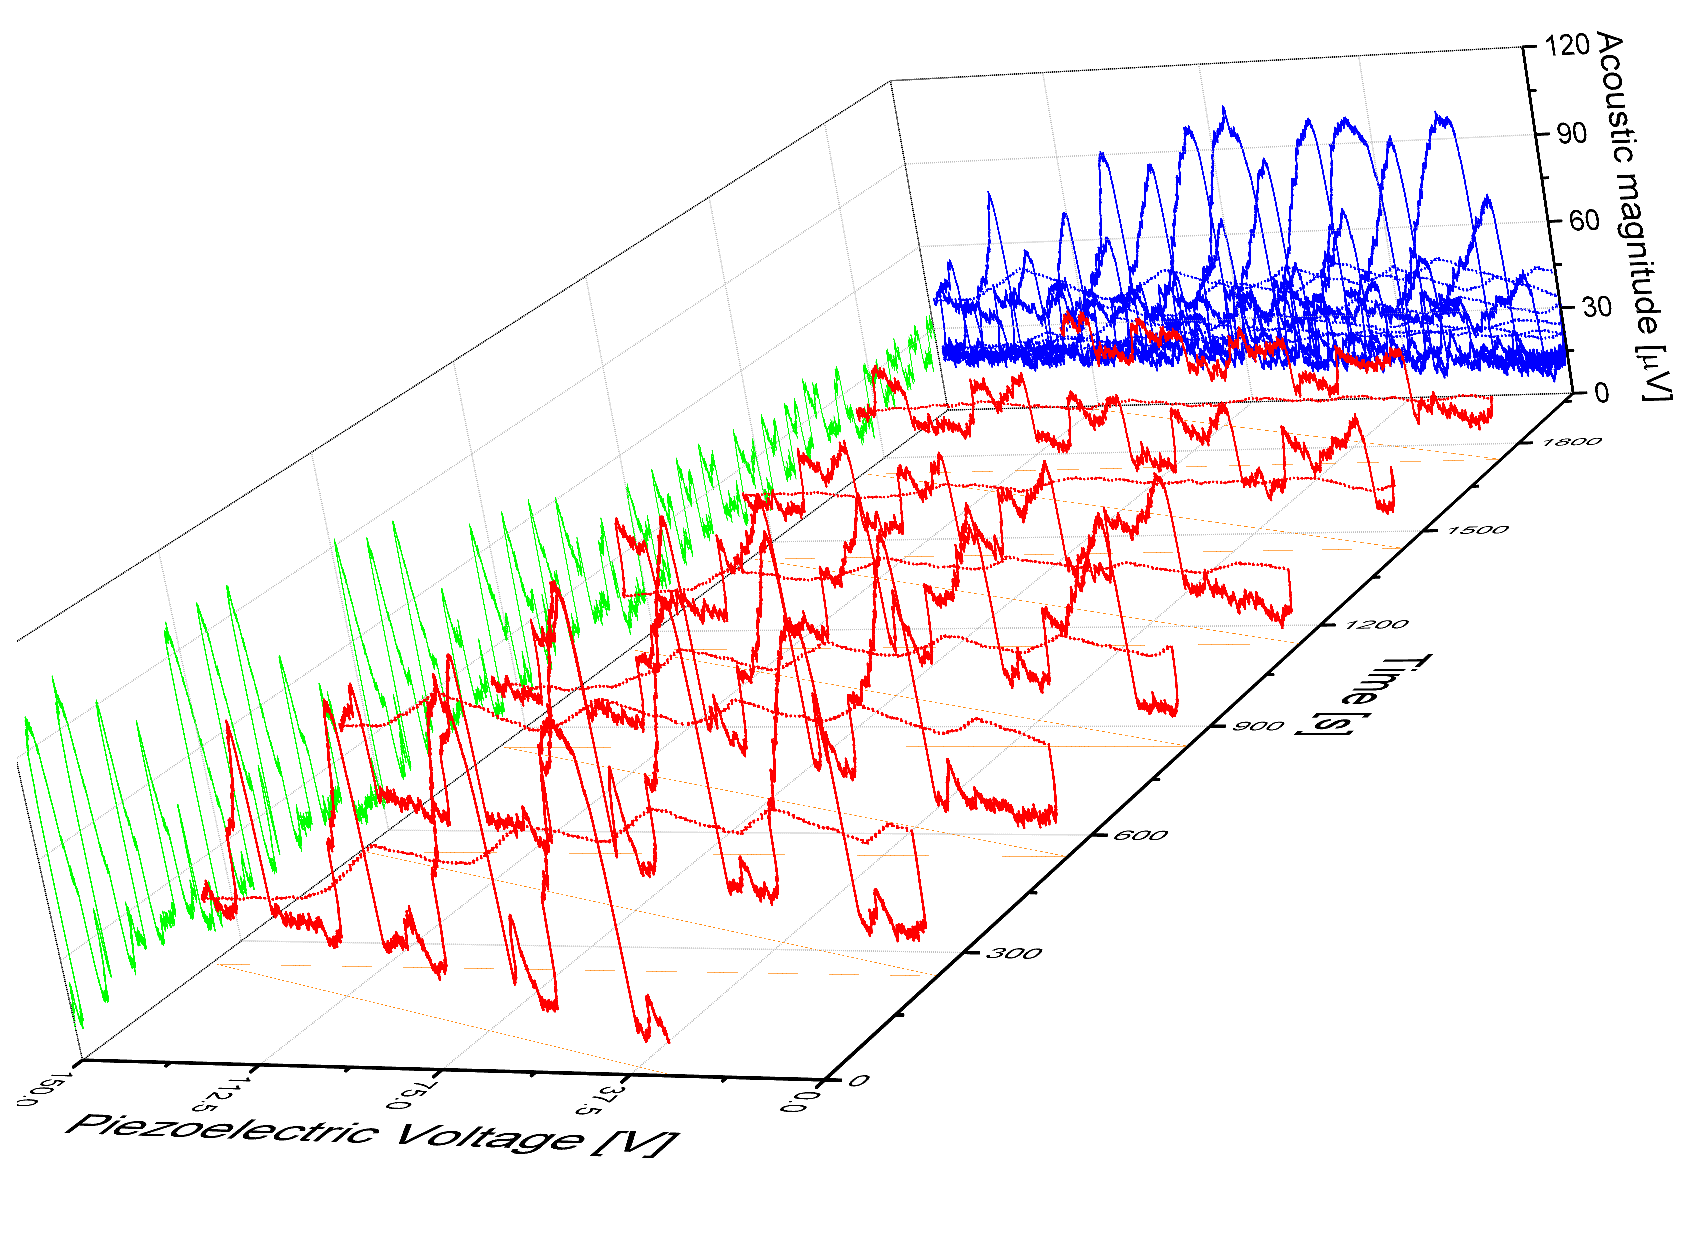
\includegraphics[height=\textheight, draft=\foto]{eps/7sweeps.eps}
\caption{In this measurement it is shown not only the fact that the peaks shift in voltage with time but can completely fade away after some minutes. Laser parameters: 25,03\cel; 80,01 mA}
\label{7sweeps}
\end{figure}\vfill
\end{landscape}
  
	\subsection{Multiple focused sweeps}\label{focus}
Another measurement methodology we used exploited repeated single-peak sweeps instead of 
full 0 to 150 V sweeps. This was intended to better study both the absorption peak shape and the evolution caused by external factors. In this kind of measurements it is also possible to use uncontrolled evolution at our advantage, since sometimes it allowed to increase the tunability range before a mode hopping. \cref{multisweep} shows how repeating a measurement of the same peak changed the part of the peak we were able to see. In \cref{multisweep1} the part of the peak we were able to see decreased after each sweep, while in \cref{multisweep2} the scanned part of the peak instead increased \textquotedblleft thanks\textquotedblright to the uncontrolled time evolution.
In both of these examples we see that we could not usually measure the "tunability range" using the spectrometer data, but still we are able to see that the voltage to laser mode dependence changes with time. 

\begin{figure}[!phtb]\centering
\subfigure[Laser parameters: 27,68\cel; 80,01 mA\label{multisweep1}]{\includegraphics[width=\linewidth, height=9.5cm, draft=\foto]{eps/multisweeps1.eps}}
\subfigure[Laser parameters: 25.03\cel; 80,01 mA\label{multisweep2}]{\includegraphics[width=\linewidth, height=9.5cm, draft=\foto]{eps/multisweeps2.eps}}
\caption{The resonance frequency shifts after every measurement, changing the part of the peak (in black) we were able to scan and decreasing the maximum measurable intensity.}
\label{multisweep}
\end{figure}

In order to better study how the voltage to wavelength output changed with time we plotted all the sweeps of \cref{multisweep1} on a voltage/intensity graphic, thus getting \cref{nonshiftedpeaks}, and subsequently shifted them by the voltage required to match the part of the peak which most likely corresponded to the oxygen absorption peak (see \cref{factorsinfluencingtheshapeofthepeaks}), getting \cref{shiftedpeaks} as result.

\begin{figure}
\subfigure[Same measurement as \cref{multisweep1}, but rearranging the data to split the 10 different sweeps.\label{nonshiftedpeaks}]{\includegraphics[width=\linewidth, height=9.5cm, draft=\foto]{eps/multiunmatched.eps}}
\subfigure[Each measurement is now shifted of the values listed below in \cref{peakshifts} in order to match the part of the peak corresponding to the oxygen absorption peak.\label{shiftedpeaks}]{\includegraphics[width=\linewidth, height=9.5cm, draft=\foto]{eps/multimatched.eps}}
\caption{In order to compare the different signal peaks, and relate them to the same absorption peak, we shifted them manually during the data processing.}
\label{grafishifti}
\end{figure}

In order to make the edges of the peak match, we had to shift the various peaks of the values listed in \cref{peakshifts}
\begin{table}[!htbp]\centering
\begin{tabular}{|c|c|c|}
\hline
N of peak & Shift [V] & $\Delta$Shift [V] \\ \hline
2 & -0.04 & -0.04 \\ \hline
3 & -0.065 & -0.025 \\ \hline
4 & -0.1 & -0.035 \\ \hline
5 & -0.12 & -0.02 \\ \hline
6 & -0.142 & -0.022 \\ \hline
7 & -0.157 & -0.015 \\ \hline
8 & -0.185 & -0.028 \\ \hline
9 & -0.195 & -0.01 \\ \hline
10 & -0.22 & -0.025 \\ \hline
\end{tabular}
\caption{Shifts of peaks in \cref{shiftedpeaks} with respect to the first peak and to the precedent peak.}
\label{peakshifts}
\end{table}

Looking at these data we could notice that, while the evolution is monotonic during our whole measurement, its speed is not constant, i.e. every peak has to be shifted a different amount with respect to the previous one.

\begin{figure}[!tphb]\centering
\includegraphics[width=\linewidth, draft=\foto]{eps/multimatchedwavelength.eps}
\caption{In this graphic the wavelength corresponding to each sweep has already been shifted of the same amount as the data in graph \cref{shiftedpeaks}.}
\label{multiwave}
\end{figure}

From the wavelength to voltage graph we can also see that, even after having shifted the sweeps in order to match the peak edges, the mode hopping from 687.35 nm (not corresponding to any absorption peak) to 687.41 nm is not happening at the same voltage in the various sweeps. This means that the environmental factors evolution cannot be modelled with a simple voltage drift (otherwise the voltage could find correction by just a voltage shift), but suffers the influence of more complicated factors.
More efforts to study this kind of evolution have been described in \cref{freedrift}.

\section{Free laser drift analysis}\label{freedrift}
\subsection{Free evolution}
To study how the evolution worked we acquired some measurements of the laser output using the spectrometer and the etalon, while keeping constant all the laser parameters (current, temperature and piezoelectric voltage). At first we took a short term measurement lasting 20 minutes. But we understood that the evolution was quite slow, and that this first measurement was too short to be meaningful. We then took a second long term measurement, lasting a night time, in order to see whether a stable regime was reached. These are shown in \cref{senzaniente}.

The first thing we noticed was that the mode hopping due to the uncontrolled evolution followed the same pattern as the mode hopping due to the piezoelectric movement (see an example in \cref{hoppattern,tabrutta}). This suggested us the idea that one of the factors which generating this evolution could be a movement of the grating of the ECDL, allegedly caused by thermal expansion of the cage system holding it. 

\begin{figure}[!hptb]\centering
\subfigure[Twenty minutes measurement. No equilibrium configuration is reached, nor clear pattern is visible. Laser parameters: 29,50 $^\circ$C; 80,00 mA.\label{senzaniente20}]{\includegraphics[width=\linewidth, height=9.5cm, draft=\foto]{eps/20minuteshops.eps}} 
\subfigure[Twelve hours measurement. A low frequency pattern appears, and this looks very similar to the mode hopping pattern due to the grating movements. Laser parameters: 25,03 $^\circ$C; 80,01 mA.\label{senzaniente12h}]{\includegraphics[width=\linewidth, height=9.5cm, draft=\foto]{eps/nighttime.eps}}
\caption{Laser free drift measurements.}
\label{senzaniente}
\end{figure} 
 
\subsection{Heating- and cooling-induced evolution}

In order to confirm the fact that the evolution depends mainly on temperature (of the cage system or of the air) effects we put a tungsten lamp near the ECDL and turned it on. As we can see from \cref{lampdrift}, turning on the lamp increased the speed of the evolution a lot. After keeping the lamp on for a while we turned it off and took another measurement. This time we observed an evolution pattern almost as fast as the one with the lamp on, but with a reverse pattern. We interpreted this a signal that the system is cooling down.

\begin{figure}[!t]\centering
\includegraphics[width=\linewidth, draft=\foto]{eps/lampandnot.eps}
\caption{During the measurements with the lamp turned on we were  eventually able to see the difference in the minimum and maximum wavelength of the same mode after some drifts, as represented in the next graphic. Laser parameters: 27,68\cel; 80,01  mA.}
\label{lampdrift}
\end{figure}

\begin{figure}[!b]\centering
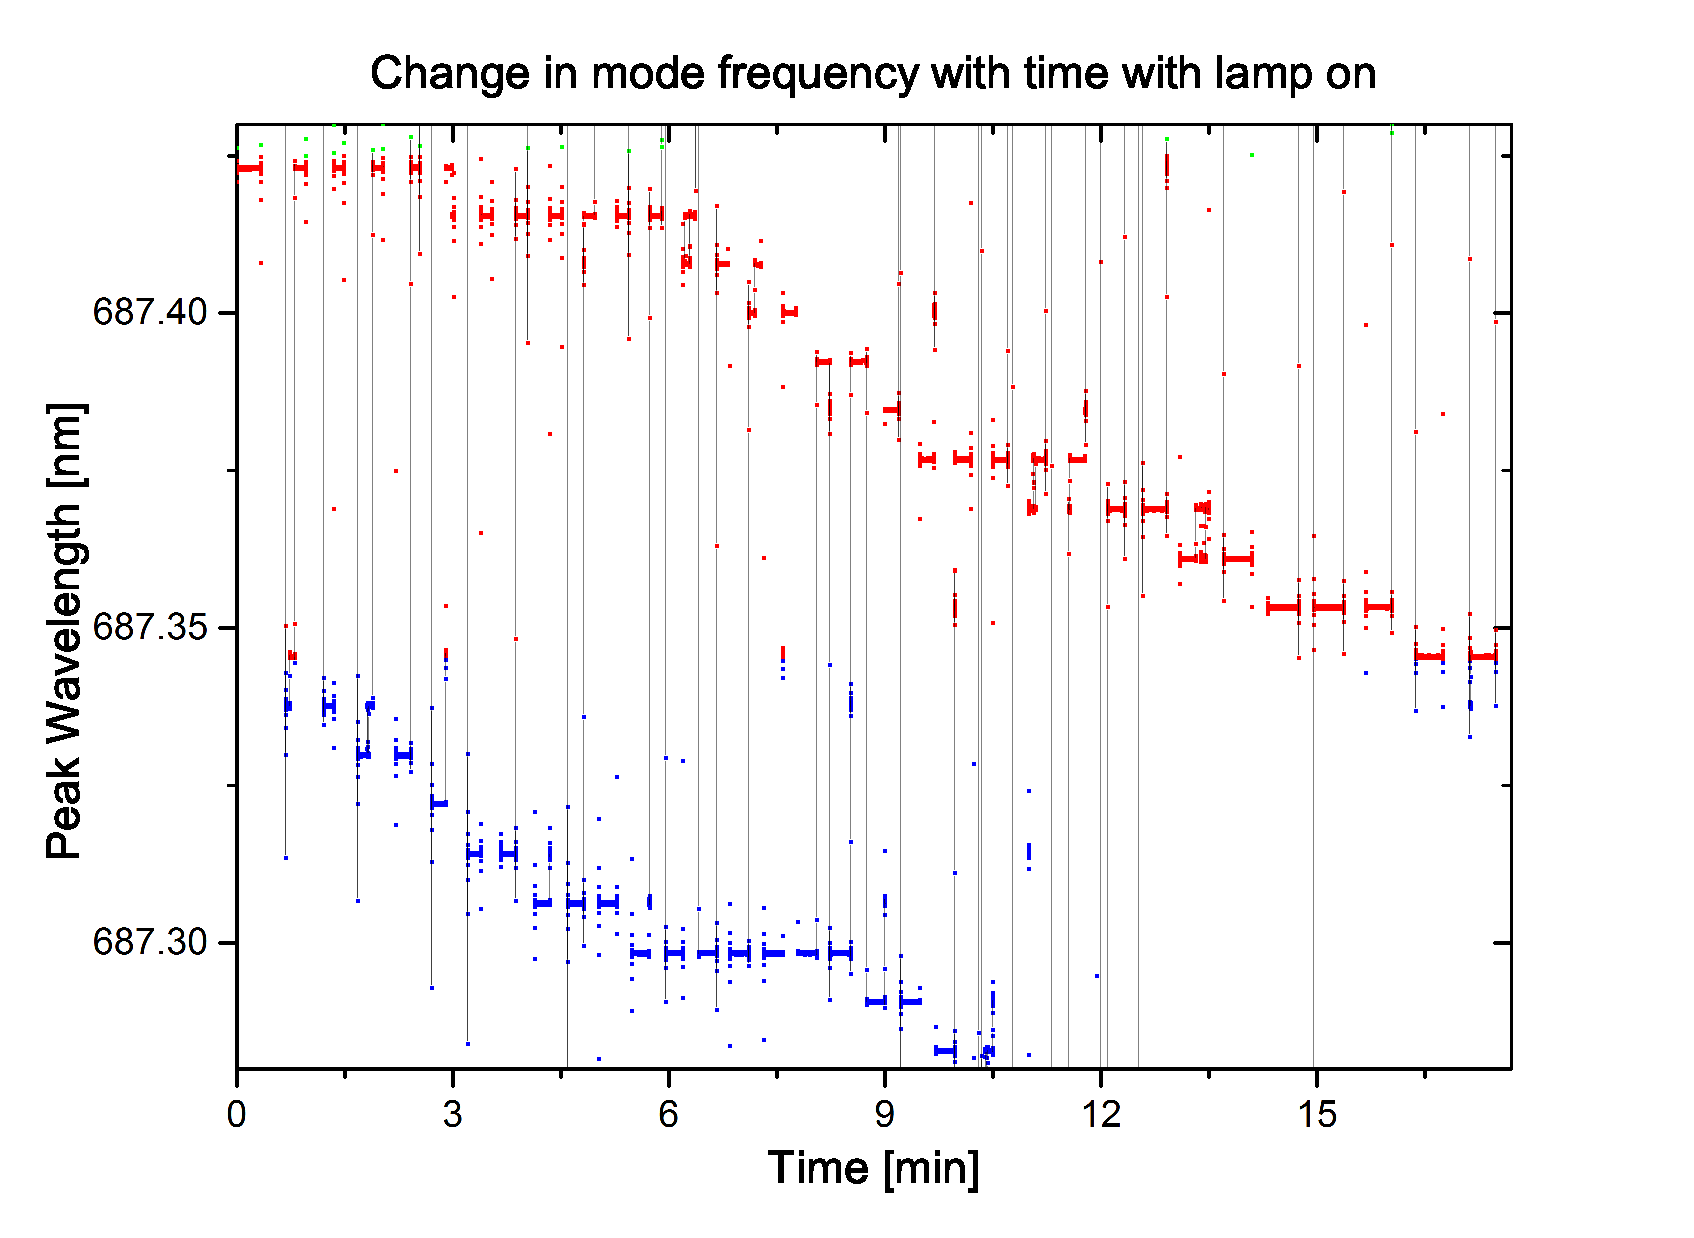
\includegraphics[width=\linewidth, draft=\foto]{eps/modedrift.eps}
\caption{The wavelength of both of the mode shown here decreases after some periods of hopping. Laser parameters: 25.03\cel; 80.01 mA.}
\label{modedrift}
\end{figure}
 
\subsection{Tunability change measurement}
Since the resolution of our spectrometer was usually not good enough to distinguish a tunability change in time, we used the etalon to take a measurement similar to the tunability measurement of a mode (687.45 nm) several times, measuring the minimum  and maximum wavelength before a mode hop for about two hours.
The results in \cref{minmaxshift} show how not only the minimum and maximum piezoelectric voltages, but also the position of the etalon interference pattern change in time. Considering that the etalon FSR is of the order of 3-4 microseconds (on the video camera PAL signal), we found that the min-max drift is of the order of about one half as the tunability found in \cref{tuna}.
%is of the order of the Ghz/timeunitnoncostante
%l'incertità dei dati dovuta alla larghezza dei picchi (che conta un tot) nella tabella è dei soliti 40ns/2radq2log2 cioè di circsa 2.12330450072005E-007 s ma forse un po' menosispera. l'errore di risoluz dell'oscillocoso sarebbe invece 40 ns /radq12).
\begin{table}[!p]
\begin{tabular}{|c|c|c|c|c|c|}
\hline
Time [min] & $\Delta$Min [ns] & Min volt. [V] & $\Delta$Max [ns] & Max volt. [V] & Tunab. [ns] \\ \hline
%0 & 9.677 & 3 & 9.678 & 17 & 560 \\ \hline
15 & 0 & 19 & 180 & 24 & 720 \\ \hline
30 & 250 & 20 & $<$40 & 27 & 500 \\ \hline
50 & 260 & 23 & 260 & 29 & 480 \\ \hline
95 & -330 & 23 & -360 & 29 & 440 \\ \hline
135 & 330 & 29 & 220 & 38 & 560 \\ \hline
\end{tabular}
\caption{Shifts of the maximum and minimum positions on the oscilloscope of the 687.45 nm mode. As discussed in \cref{tuna}, the uncertainty on the time measurement is estimated to be $\simeq$ 40 ns.}
\label{minmaxshift}
\end{table}


	\clearpage
	\appendix\addcontentsline{toc}{chapter}{APPENDIX}

	\chapter{Extended Cavity Diode Laser (ECDL)}\label{ECDL}
	\section{Introduction to LD tuning}

The light emitted by a diode laser is often practically useless to an experimentalist because of several different reasons:
\begin{itemize}
 \item greatly diverges in an oval shape pattern
 \item because of the small cavity of the laser it has a larger bandwidth which means that diode lasers emit light over a broader range of wavelengths than other kinds of lasers
 \item could have an unstable wavelength due to temperature or current fluctuations.
\end{itemize}

The first problem makes it necessary to collimate the output of the diode laser, that is, bend the diverging light through a lens (or several lenses) so that all the output goes in one direction. One can achieve this result by using a single lens as long as the laser is placed exactly at the focal  point of the lens one chooses. The focal point of a lens is also the point through which all light parallel to its normal axis will converge. Hence, if we place our diode laser at the focal point of our collimating lens all light from the diode laser that passes through the lens will exit parallel to the normal axis and all light that enters the face of the lens at normal incidence will be focused the diode laser.

The broad linewidth of solitary diode laser often reduces their usefulness for spectroscopy applications. To overcome this problem several techniques have been developed, for example:
\begin{itemize}
\item negative electronic feedback
\item resonant optical feedback from a high-finesse optical cavity
\item extended-cavity configurations
\end{itemize}
Among all these techniques that can be used to reduce the laser linewidth down to the kHz range, the extended-cavity configuration with grating feedback has become the most popular. It provides a simple mean to achieve a wide wavelength tuning range and a narrow linewidth.
The external cavity could also solve the instability through optical feedback, severely reducing mode hoping.
In our experiment we used an external cavity in Littrow configuration so we will focus on explaining how such a cavity and it's main components work.
A schematic layout of the extended-cavity laser is outlined in \cref{grating}. The laser system consists of a diode laser as the active medium, a collimating lens and a diffraction grating. The external cavity is formed between the rear facet of the diode laser and the grating as a wavelength selective mirror. The laser frequency depends critically on the optical length of the cavity, which is sensitive to any changes in the refractive index of the cavity media (diode laser, lens, and air) and to changes in the physical cavity length.
The collimation lens of the ECDL (Extended Cavity Diode Laser) is one critical part of attaining optical feedback. The second part of our system that allows optical feedback is the diffraction  grating. 

\begin{figure}[!hbt]\centering
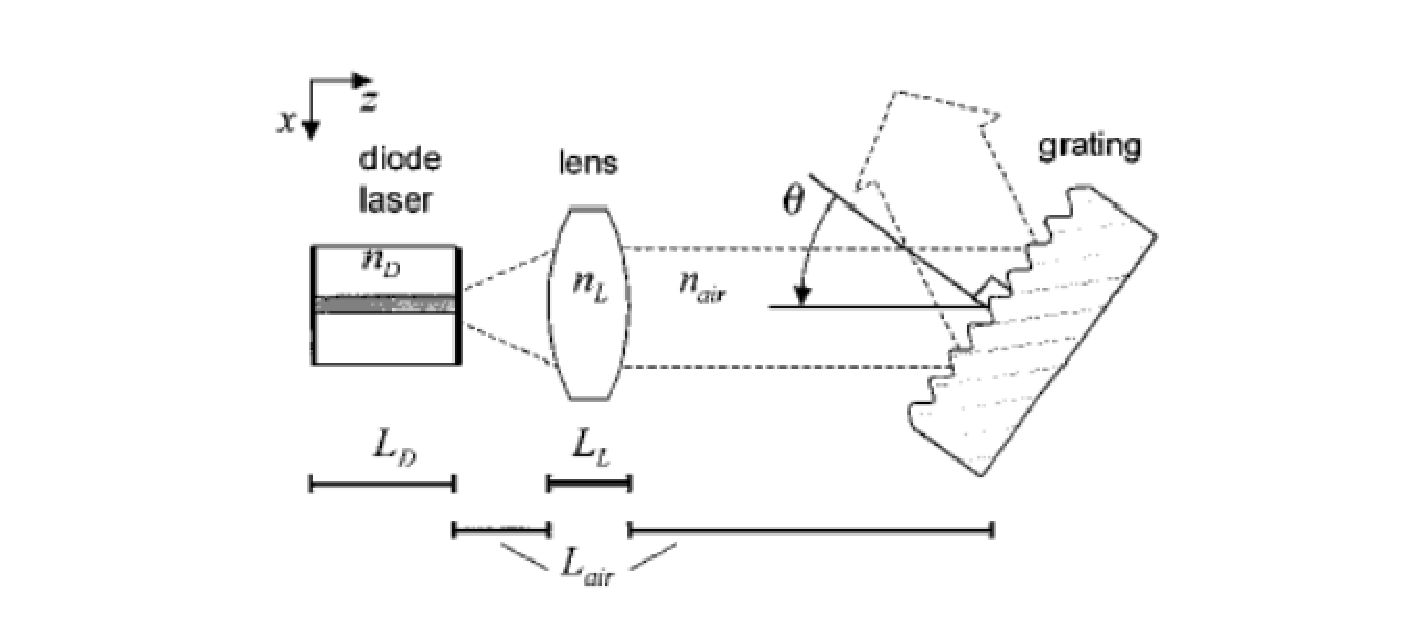
\includegraphics[width=\linewidth, draft=\foto]{eps/littrow1.eps}
\caption{Schematic layout of the extended cavity laser. The total optical path length in the cavity is $L_{\mai{ec}}=L_{\mai{d}}n_{\mai{d}}+L_{\mai{l}}n_{\mai{l}}+L_{\mai{air}}n_{\mai{air}}$}
\label{grating}
\end{figure}

    \section{Diffraction theory for a grating}\label{gratingtheory}
A diffraction grating is a finely scored reflective material that, due to its geometry, allows only certain wavelengths of light incident at an angle to interfere constructively with itself as it is reflected outwards.


 The light diffracted by each groove combines to form a diffracted wavefront. Diffraction by a grating can be visualized from the geometry in \cref{littrow4}, which shows a light ray of wavelength $\lambda$ incident at an angle $\alpha$ and diffracted by a grating along angles $\beta_{\mai{m}}$. These angles are measured from the grating normal, which is the dashed line perpendicular to the grating surface at its center. The sign convention for these angles depends on whether the light is diffracted on the same side or the opposite side of the grating as the incident light. In \cref{littrow3a}, which shows a reflection grating, the angles are  $\alpha>0$ and $\beta_{\mai{1}}>0$ (since they are measured counter-clockwise from the grating normal), while we have $\beta_{\mai{0}}<0$ and $\beta_{\mai{-1}}<0$ (since they are measured clockwise from the grating normal). Diagram \cref{littrow3b} shows the case for a transmission grating.
\begin{figure}[!bht]\centering
\subfigure[A reflection grating: the incident and diffracted rays lie on the same side of the grating.\label{littrow3a}]{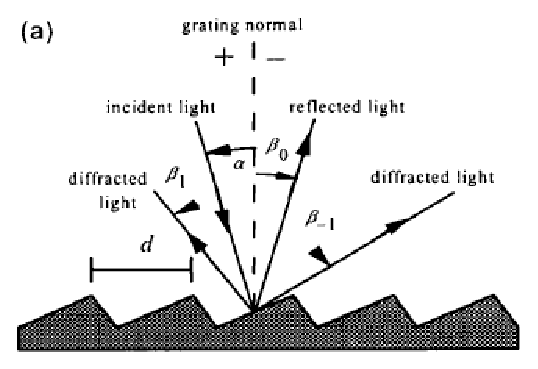
\includegraphics[width=.46\linewidth, draft=\foto]{eps/littrow3a.eps}}
\hfill
\subfigure[A transmission grating: the incident and diffracted rays lies on opposite sides of the grating.\label{littrow3b}]{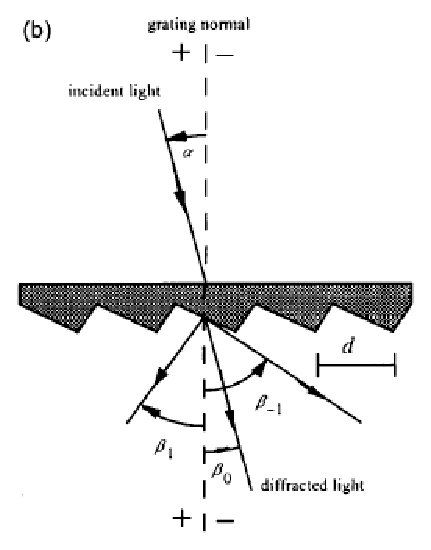
\includegraphics[width=.46\linewidth, draft=\foto]{eps/littrow3b.eps}}
\caption{A comparison between reflection and transmission grating.}
\end{figure}

The formula for constructively diffracted orders of light reflected from a diffraction grating is:(VERIFICO NOMI DEGLI ANGOLI!!!111!!!!111!!!1111)
\mate
d\sin\theta=m\lambda
\label{gianfrancioschio}
\atem
where $d$ is the spacing between reflective surfaces, $\theta$ is the angle of incidence, $\lambda$ is the wavelength of the incident light and $m$ is an integer. One consequence of the above equation is that spectra diffracted off a grating are reproduced at several different angular positions about the grating. The various replications of the spectra are called \textit{orders of diffraction} and obey the following relationship 
\mate
\sin\theta_{\mai{i}} + \sin\theta_{\mai{m}}= N m \lambda
\atem
where $\theta_{\mai{m}}$ is the angle of the $m$th order diffracted beam, $N$ is the spatial frequency of the grating (units mm$^{-1}$), and $\theta_{\mai{i}}$ and $\lambda$ are the incident light angle and wavelength respectively.

When monochromatic light impinges on a grating surface, it is diffracted into discrete directions.
We can easily calculate the  separation between these directions by inverting /ref{gianfrancioschio}.
\mate
\beta[\lambda]=\arcsin\left[\frac{m\lambda}{d} – \sin\alpha\right]
\atem
When $m=0$, the grating acts as a mirror, and the wavelengths are not separated ($\beta=-\alpha$ for all $\lambda$); this is called specular reflection or \textit{the zeroth order}. 
\begin{figure}[!htb]\centering
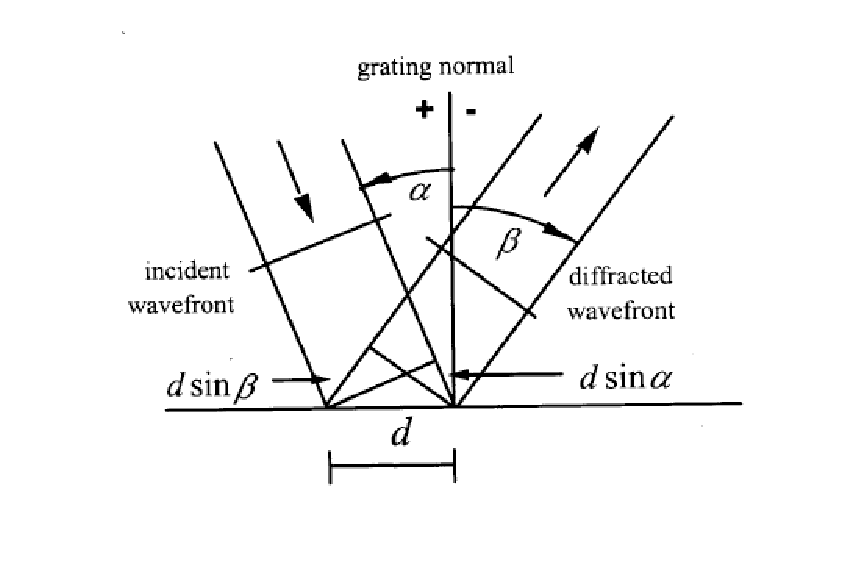
\includegraphics[width=\linewidth, draft=\foto]{eps/littrow4.eps}
\caption{Geometry of diffraction, for planar wavefronts.}
\label{littrow4}
\end{figure}

\section{Littrow configuration ECDL}\label{Littrowsection}
In the Littrow configuration for the external cavity, shown in \cref{littrow2}, the grating is aligned in way such that the first order diffraction from the grating is coupled directly back into the laser, while the zeroth-order diffraction is reflected as the output beam. The lasing wavelength is dependent on the angle of the incident laser beam with respect to the grating, otherwise known as the Littrow angle $\theta$.
There are 3 cavities which set up such configuration:
\begin{enumerate}
\item Laser diode cavity or internal Fabry-P\'{e}rot cavity
\item External cavity between grating and back side of the diode 
\item Parasitic cavity between grating and the front facet of the diode
\end{enumerate}

\begin{figure}[!t]
\centering
%\mbox{
%\begin{minipage}[b]{.60\textwidth}
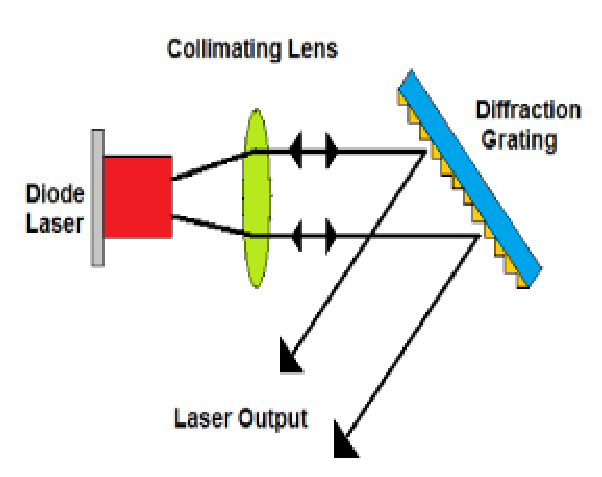
\includegraphics[width=0.7\linewidth, height=5cm, draft=\foto]{eps/littrow2.eps}
%\end{minipage}
%\begin{minipage}[b]{.35\textwidth}
\caption{Schematic diagram of external cavity in Littrow configuration.}
\label{littrow2}
%\end{minipage}}
\end{figure}

The key to the Littrow configuration is the backcoupling of the first-order diffraction beam from the grating into the laser diode. Without this feedback, the Littrow laser cannot achieve single-mode emission and will lase at a wavelength set by the gain peak of the semiconductor active region. When the feedback beam is well aligned, interference fringes are expected in the output beam and the laser remains in single-mode despite small temperature and current changes.

	\section{Main sources of noise in a ECDL}
The frequency of a solitary diode laser is sensitive to variations in the injection current and the junction temperature. This is mainly caused by changes in the refractive index of the active medium and in the optical gain. 
These effects can be reduced in an ECDL but other many noise factors are introduced due to the instability of the optical length of the external cavity.
We will now summarize the main factors which influence the optical length of the cavity.

The optical length of the collimating lens changes with temperature. This is caused by thermal expansion of the material and temperature dependence of the refractive index. Their effects on the laser frequency are described by the relationship 
\mate
\frac{d\nu}{dT_{\mai{l}}}=-\nu\frac{L_{\mai{l}}}{L_{\mai{ec}}}\alpha_{\mai{l}}\left(n_{\mai{l}}-n_{\mai{air}}+\beta_{\mai{l}}n_{\mai{l}}\right)
\label{effect1}
\atem
where $n_{\mai{l}}$ and $n_{\mai{air}}$ are the refractive indices of the lens material and air respectively, and $L_{\mai{l}}$ and $L_{\mai{ec}}$ are the physical length of the lens and the total optical path length of the external cavity, respectively. The thermal expansion coefficient of the lens material is denoted by $\alpha_{\mai{l}}$ and the relative temperature coefficient of the refractive index by $\beta_{\mai{l}}$. 

The refractive index of air is mainly sensitive to variations in pressure $p$ and temperature $T_{\mai{air}}$.The variations in the laser frequency due to these changes are described by
\begin{align}
\frac{d\nu}{dp}=-\nu\frac{L_{\mai{air}}}{L_{\mai{ec}}}\frac{dn_{\mai{air}}}{dp}\label{effect2}\\
\frac{d\nu}{dT_{\mai{air}}}=-\nu\frac{L_{\mai{air}}}{L_{\mai{ec}}}\frac{dn_{\mai{air}}}{dT_{\mai{air}}}
\label{effect3}
\end{align}
where $L_{\mai{air}}$ is the cavity length containing air.	

The mechanical structure of the cavity often contains micrometric screws and piezoelectric transducers (PZTs) for wavelength control. The sensitivity of the laser frequency to thermal expansion of these parts can be written as
\mate
\frac{d\nu}{dT_{\mai{m}}}=\pm\nu\frac{L_{\mai{m}}}{L_{\mai{ec}}}\alpha_{\mai{m}}
\label{effect4}
\atem
where $L_{\mai{m}}$ and $\alpha_{\mai{m}}$ are the length and the thermal expansion coefficient of the mechanical part, respectively.

A transverse displacement along $x$ axis of the collimating lens with respect to the laser diode changes the beam direction. This causes a frequency shift due to a change in the cavity length. For a small displacement, the frequency shift can be written as
\begin{align}
\frac{d\nu}{dx}=\frac{\nu\tan\theta}{f_{\mai{l}}}
\label{displacement}\\
\frac{d\nu_{\mai{g}}}{dT}=-\nu_{\mai{g}}\alpha_{\mai{g}}
\label{displacement2}
\end{align}
where $f_{\mai{l}}$ is the focal length of the lens and $\theta$ is the angle between the grating normal and the incident beam, while $\nu_{\mai{g}}$ and $\alpha_{\mai{g}}$ are the central frequency of the grating feedback and the grating thermal expansion coefficient respectively. The displacement of the lens can be caused, for example, by asymmetric thermal expansion relative to the optical axis or by mechanical vibration of the lens holder. 

There are additional effects that influence mainly the short-term frequency stability of the laser: current- and PZT driver noise, mechanical vibrations, acoustic disturbances, and rapid changes in the refractive index of air caused by air flow. All of these factors have an effect on the length of the external cavity and, consequently, generate frequency modulation of the laser.
	\chapter{The lock-in amplifier}\label{lokkin}
	\section{Basic theory}

A lock-in amplifer is a device used to extract a frequency modulated narrow band signal from a noisy environment by using a phase sensitive detector. The output will typically be a DC voltage which is proportional to the original signal amplitude. The device has two inputs as shown in \cref{lockin1}. One is the input signal that is to be measured, the other is the frequency reference. The reference should have the same frequency as the modulation of the original signal. This signal is usually a sync-signal originating from the same source as the input signal modulator (in our experiment this is the optical chopper). 

The input signal of the lock-in is first passed through an amplifier of gain $g$, which is adjustable and is used to control the sensitivity of the lock-in. The reference signal instead is led through a sine-former, i.e.  a block consisting of many components which transform the signal to ensure it has sinusoidal form and a specific predetermined amplitude.

\begin{figure}[!hbt]\centering
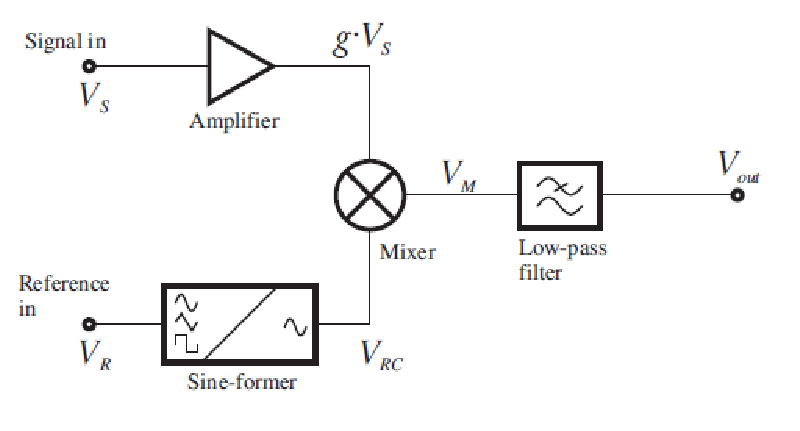
\includegraphics[width=\linewidth, draft=\foto]{eps/lockin1.eps}
\caption{Block scheme of a lock-in amplifier.}
\label{lockin1}
\end{figure}

The following \cref{sinusoidal} states the  modulated input signal $K[t]$ if we assume it is sinusoidally modulated \footnote{Of course this is not out case, but thanks to Fourier decomposition we can think of any generic signal as a sum of sinusoidal components.}, where $f$ is the frequency of the carrier, while \cref{reference} states the reference signal after it has passed through the sine-former, and assuming it has the exact same frequency $f$ as the input signal.

\begin{align}
V_{\mai{s}}=K[t]\cos[2\pi ft+\phi_{\mai{s}}]
\label{sinusoidal}\\
V_{\mai{rc}}=\cos[2\pi ft+\phi_{\mai{r}}]
\label{reference}
\end{align}
The mixer then combines these two signals by multiplying them, giving
\begin{align}
V_{\mai{m}}&=K[t] g\cos[2\pi ft+\phi_{\mai{s}}]\cos[2\pi ft+\phi_{\mai{r}}]\nonumber\\
&=\frac{1}{2}K[t]g\left(\cos[\phi_{\mai{s}}-\phi_{\mai{r}}]+\cos[2\pi\cdot2ft+\phi_{\mai{s}}+ \phi_{\mai{r}}]\right)\label{mixer}
\end{align}

As can be seen in \cref{mixer}, assuming the bandwidth of the input signal $K[t]$ is much smaller than the carrier frequency, the result consists of two frequency components. One at zero (DC), and one at the double of the carrier frequency. If the low pass filter is set correctly the double frequency component will be completely removed, and the output is therefore as stated by
\mate
V_{\mai{out}}=\frac{1}{2}K[t]g\cos\left[\phi_{\mai{s}}-\phi_{\mai{r}}\right]
\atem

We can see that the output is a DC voltage which is proportional to the original signal amplitude $K[t]$. The amplifier gain $g$ is such that, when assuming  $\phi_{\mai{s}}=\phi_{\mai{r}}$, the output is 10V if the RMS-value of the input signal is the same as the sensitivity-setting. For lower input signals, the output is proportionally lower, and a higher input would eventually overload the lock-in. In most lock-in amplifiers, the sensitivity can be tuned according to the characteristics of the input signal.

	\section{Dual lock-in amplifier}
	In the single lock-in amplifier we just studied, the output signal not only depends on the amplitude of the original signal, but also 
	on the phase difference between the modulation and the reference signal given to the amplifier, which in principle could be unknown or unstable.
	In order to solve such a problem the dual lock-in amplifier was implemented.
	The dual lock-in amplifier has two mixers with dedicated low pass filters. One of these mixers multiplies the reference and the input signal like in the single lock-in amplifier, while the other one multiplies the input signal with the reference phase shifted by 90\textdegree. \cref{lockin2} illustrates this principle.

\begin{figure}[!hbt]\centering
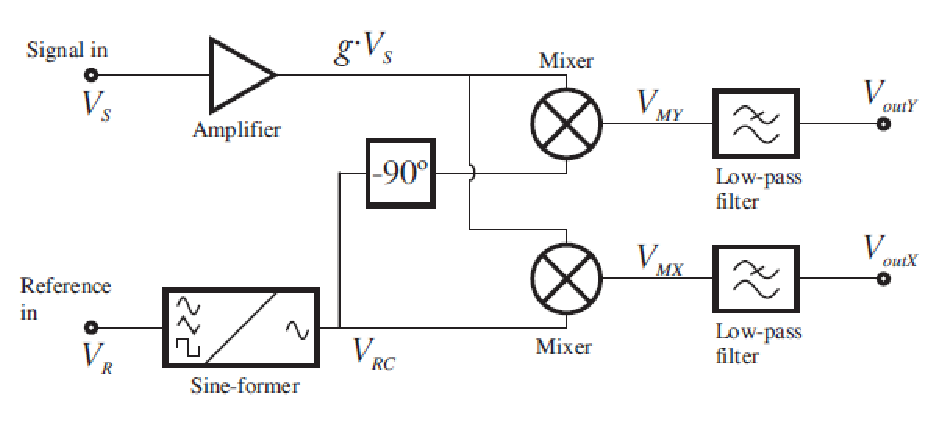
\includegraphics[width=\linewidth, draft=\foto]{eps/lockin2.eps}
\caption{A dual lock-in amplifier}
\label{lockin2}
\end{figure}

The two outputs then become

\begin{align}
V_{\mai{out}}^{\mai{x}}&=\frac{1}{2} K[t] g\cos\left[\phi_{\mai{s}}-\phi_{\mai{r}}\right]
\\
V_{\mai{out}}^{\mai{y}}&=\frac{1}{2} K[t] g\sin\left[\phi_{\mai{s}}-\phi_{\mai{r}}\right].
\end{align}

$V_{\mai{out}}^{\mai{x}}$ is called the in phase component of the output, while $V_{\mai{out}}^{\mai{y}}$ is called the quadrature component. For convenience it could be useful to define a new complex quantity $V_{\mai{out}}^{\mai{cp}}$ like

\mate
V_{\mai{out}}^{\mai{cp}}=V_{\mai{out}}^{\mai{x}}+iV_{\mai{out}}^{\mai{y}}
\atem

No matter what the phase difference between the input and the reference is, the magnitude of $V_{\mai{out}}^{\mai{cp}}$ doesn't depend on the phase difference and can now be used to find the amplitude of the input signal modulated at frequency $f$ .

	\section{Low-pass filter}

The low pass filters in \cref{lockin1,lockin2} are supposed to remove the double frequency component in \cref{mixer}. In addition, these filters may remove a lot of additional noise which unavoidably adds to the signal during the elaboration and trasmission of the signal. \cref{lockin3} shows an example of why the low pass filter is useful. Here the mixing process causes a shift in the spectrum such that the desired signal is shifted to $f=0$ (DC). The dotted line represents the frequency response of the filter, and should be multiplied with the input signal to give the output. All the noise which is not within the bandwidth of the filter is removed.

In most lock-in amplifiers the low-pass filter is adjustable through two parameters. One of them is the time constant $\tau$. If the input were to suddenly change, this is the time it would take before the output is adjusted to 63\% of this change. The second parameter is the number of such filters which influences the resulting cut-off slope. Between one and four filters with the same time constant $\tau$ can be cascaded to form a sharper filter.

\begin{figure}[!hbt]\centering
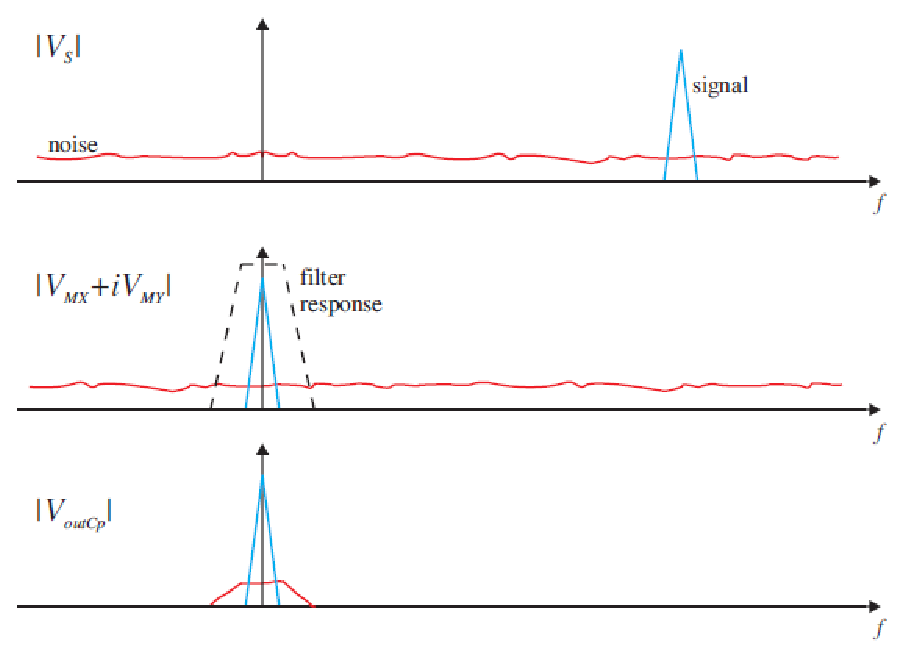
\includegraphics[width=\linewidth, draft=\foto]{eps/lockin3.eps}
\caption{The low pass filter removes all the noise which is not within the bandwidth of the filter.}
\label{lockin3}
\end{figure}
	\section{The etalon}
\subsection{Introduction}
The etalon is an optical device made of two perfectly parallel semi-reflecting surfaces. It can be thought as a Fabry-P\'erot cavity which walls are fixed. This geometry can be implemented either with an air-based or a solid design. The first one consist in two surfaces separated by air, one of which usually can be moved via piezoelectric actuators. The second one is just made from a piece of glass (or other materials suitable for the desired application) with a partially reflecting coating covered facets (\cref{solidstate}). While the air based etalons make longer cavities, thus more precise, they are extremely delicate and cumbersome to manage, mostly because the two surfaces must be kept parallel within hundredths of wavelength. The solid state ones, on the other hand, are usually smaller and less performing, but way more robust and easier to use.

Every time the impinging beam encounters one of the two optical surfaces the light is partially reflected and partially transmitted. Multiple reflections occur inside the two surfaces leading to an infinite number of rays departing from the interferometer in both the transmitted and reflected directions. Contiguous beams differ for a constant phase and this causes an interference pattern, as shown in \cref{etalonmonitor}.

\begin{figure}[!h]\centering
\begin{minipage}[t]{0.46\textwidth}\centering
\includegraphics[width=\linewidth, height=5cm]{eps/etalon5.eps}
\caption{Solid state etalons.}
\label{solidstate}
\end{minipage}
\hfill
\begin{minipage}[t]{0.46\textwidth}\centering
\includegraphics[width=\linewidth, height=5cm]{eps/thering.eps}
\caption{The etalon diffraction pattern seen through our videocamera.}
\label{etalonmonitor}
\end{minipage}
\end{figure}

\subsection{Theoretical treatment}
To derive the phase difference between two adjacent beams, let's begin calculating the difference in their optical paths (\cref{fig:angoli}). We thus choose two parallel beams, such as $OB$ and $CD$, and draw a wavefront perpendicular to them, $AC$. 
\begin{figure}[!h]
\centering
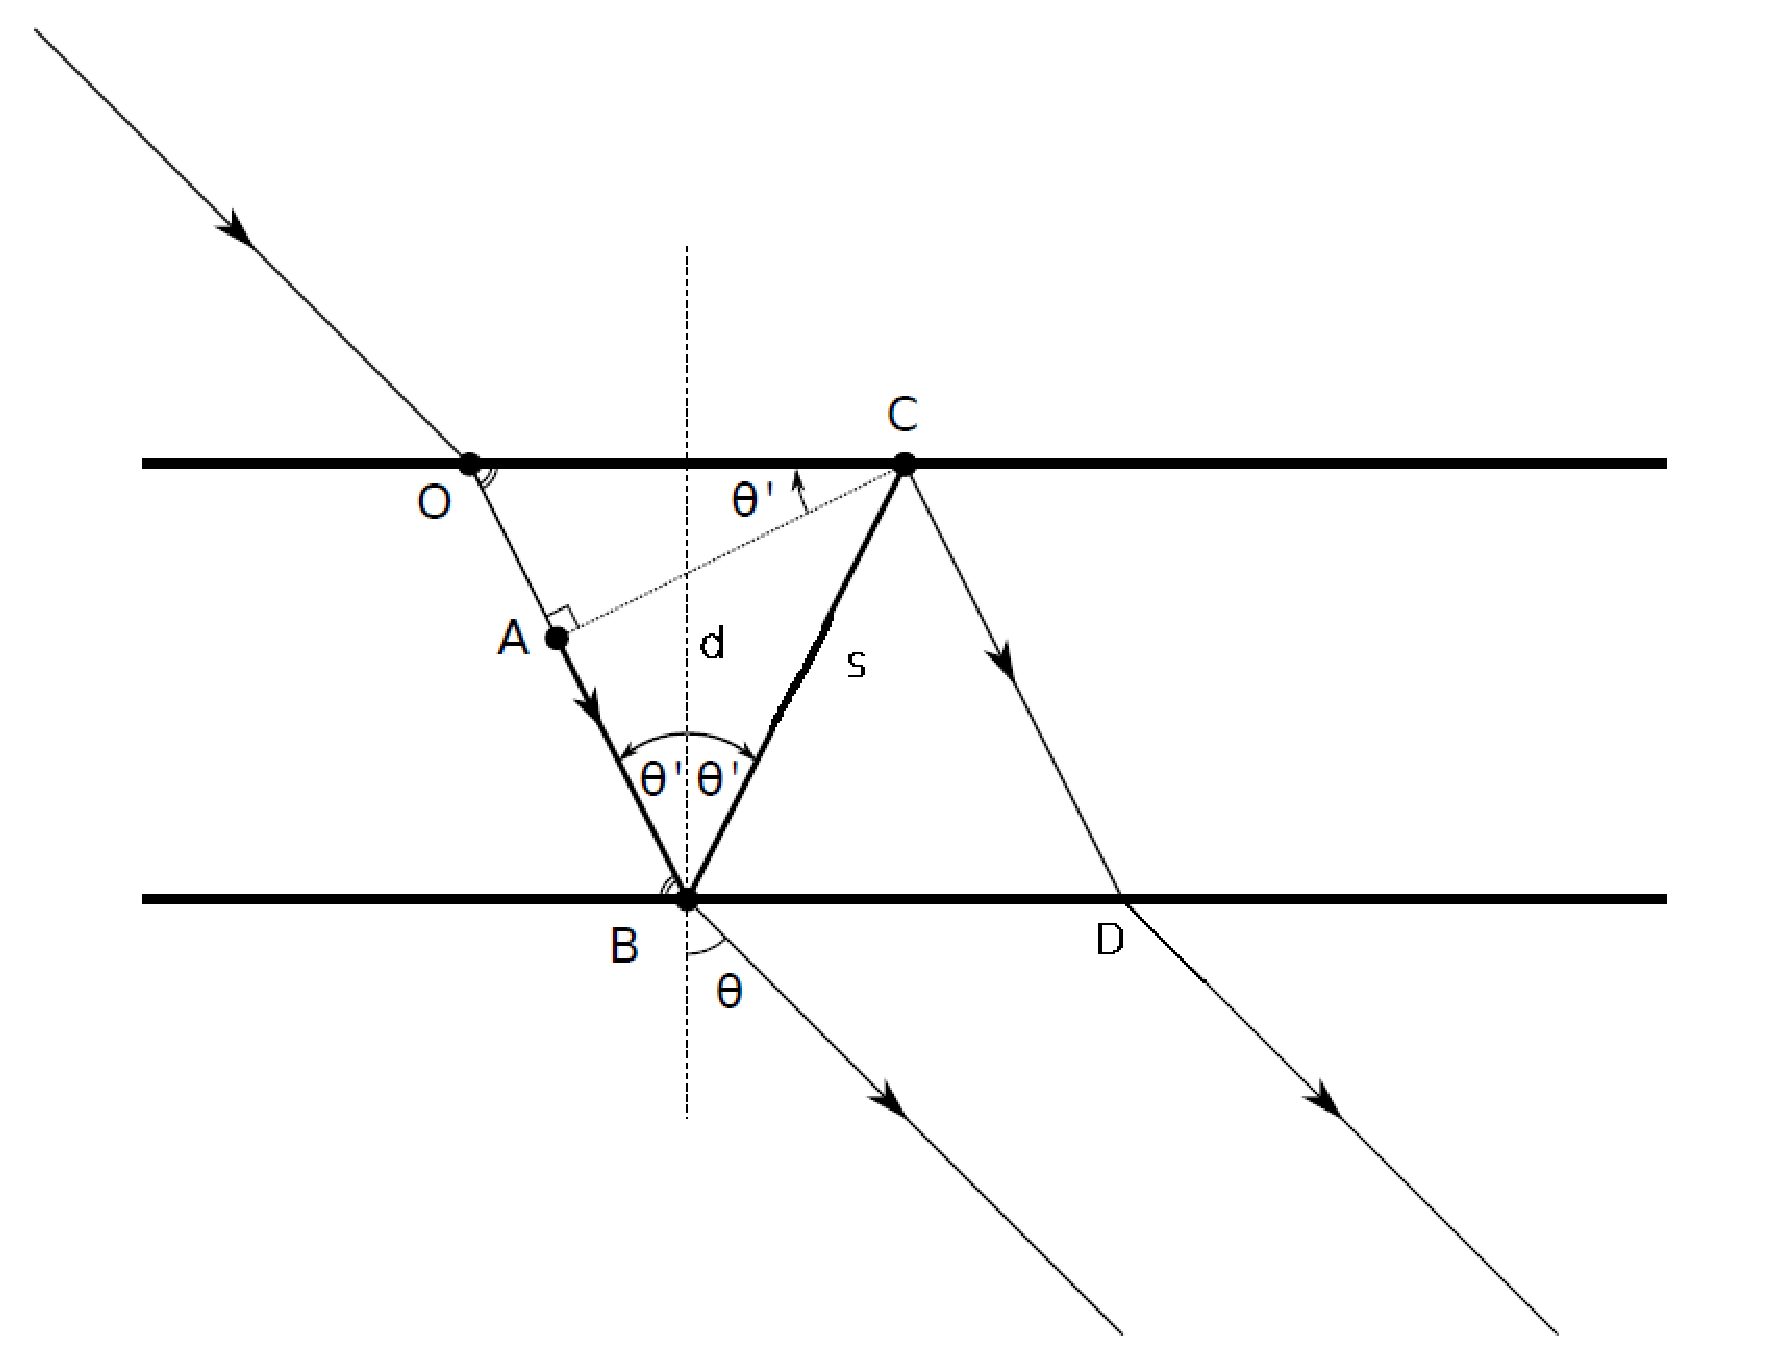
\includegraphics[width=.8\linewidth]{eps/angoli.eps}
\caption{The impinging beam changes direction due to refraction index difference between the air and the glass, the angles $\theta$ and $\theta'$ being related to the refraction indices $n$ and $n'$ by Snell's law.}
\label{fig:angoli}
\end{figure}
The optical path difference between $A$ and $C$ is given by
\begin{equation}
\overline{ABC}=\overline{AB}+\overline{BC}
\end{equation}
 We call $d$ the width of the etalon, and $s$ the distance traveled by the beam from one surface to the other one, so that
\begin{equation}
\overline{BC}=\overline{OB}\equiv s=\frac{d}{\cos\theta'}.
\end{equation} 
From elementary geometry considerations we get the following relationships:
\begin{eqnarray}
\overline{AB}&=&\overline{OB}-\overline{OA}\\
\overline{OA}&=&\sqrt{\overline{OC}^2-\overline{AC}^2}\\
\overline{OC}&=&2s\sin\theta'\\
\overline{AC}&=&s\sin(2\theta')
\end{eqnarray}
Then we write
\begin{eqnarray}
\nonumber\overline{OA}&=&\sqrt{4s^2\sin^2\theta'-s^2\sin^2(2\theta')}\\
\nonumber&=&\sqrt{4s^2\sin^2\theta'\left(1-\frac{\sin^2(2\theta')}{4\sin^2\theta'}\right)}\\
\nonumber&=&2s\sin\theta'\sqrt{1-\cos^2\theta'}\\
&=&2s\sin^2\theta'
\end{eqnarray}
Putting all together we get the optical path difference

\begin{eqnarray}
\nonumber\overline{ABC}&=&\overline{AB}+\overline{BC}\\
\nonumber&=&\overline{OB}-\overline{OA}+\overline{BC}\\
\nonumber&=&s-2s\sin^2\theta'+s\\
\nonumber&=&2s(1-\sin^2\theta')\\
\nonumber&=&2s\cos^2\theta'\\
&=&2d\cos\theta'.
\end{eqnarray}

If the incident light has wavelength $\lambda_0$ in the vacuum and the etalon medium has refractive index $n'$, the light wave vector inside the medium is
 \begin{equation}
k=\frac{2\pi}{\lambda_0}n'
\end{equation}
and the phase shift between two adjacent rays is 
\mate
\Delta=k\cdot\overline{ABC}=\frac{4\pi}{\lambda_0}n'd\cos\theta'
\label{phase}
\atem

Now, indicating by $T$ the overall etalon transmission coefficient and by $R$ the reflection coefficient correspondig to one round-trip, the total amplitude of the electric field in some point after the etalon is the sum of those of the subsequent rays
\mate
E_T=E_0T+E_0TRe^{i\Delta}+E_0TR^2e^{i2\Delta}+E_0TR^3e^{i3\Delta}+\dots
\atem
which is nothing but the geometrical series, that can be summed up ($|Re^{i\Delta}|<1$) to yield 
\mate
E_T=E_0T\sum_{j}\left(Re^{i\Delta}\right)^j=\frac{E_0T}{1-Re^{i\Delta}}
\atem

What we observe is actually the transmitted intensity 

\mate
I_T=|E_T|^2=|E_0|^2\frac{T^2}{|1-Re^{i\Delta}|^2}
\atem

The denominator can be rewritten as
\begin{eqnarray}
|1-Re^{i\Delta}|&=&(1-Re^{i\Delta})(1-Re^{-i\Delta})
\nona 1-R(e^{i\Delta}+e^{-i\Delta})+R^2
\nona 1-2R\cos\Delta+R^2
\nona 1-2R\left(1-2\sin^2\frac{\Delta}{2}\right)+R^2
\nona 1-2R+4R\sin^2\frac{\Delta}{2}+R^2
\nona\nonumber (1-R)^2+4R\sin^2\frac{\Delta}{2}\\
&=& (1-R)^2\left(1+\frac{4R}{(1-R)^2}\sin^2\frac{\Delta}{2}\right)
\end{eqnarray}

So that the transmitted intensity becomes
\mate
I_T=I_0\frac{T^2}{(1-R)^2}\frac{1}{\left(1+\frac{4R}{(1-R)^2}\sin^2\frac{\Delta}{2}\right)}
\label{intensity}
\atem

One defines a \textit{peak constant}
\mate
C_{\mbox{peak}}\equiv\frac{T^2}{(1-R)^2}
\atem

which is equal to 1 for an ideal surface such that $1=R+T$. In a real surface, instead, some absorption $A$ is present, so that $1=R+T+A$. The peak constant in this case can be rewritten as
\mate
C_{\mbox{peak}}=\frac{(1-A-R)^2}{(1-R)^2}=\left(1-\frac{A}{1-R}\right)^2
\atem 

Furthermore we shall define the \textit{coefficient of finesse}\footnote{Not to be confused with the \textit{finesse} defined further in this discussion at pg.\ \pageref{finesse}. These two parameters are strongly correlated, though, and literature is not uniform on which of the two is to be called "finesse".}
\mate
F\equiv\frac{4R}{(1-R)^2}.
\atem

In the ideal etalon case we have $A\simeq0$, which implies $C_{\mbox{peak}}\simeq1$,  so that \cref{intensity} eventually reduces to
\mate
I_T=I_0\ \frac{1}{1+F\sin^2\frac{\Delta}{2}}
\atem

The transmitted intensity is thus given by the constant input intensity value, modulated by the so called \textit{Airy function} plotted in \cref{Airyplot}
\mate
\frac{I_T}{I_0}=\frac{1}{1+F\sin^2\frac{\Delta}{2}}\equiv A[F;\Delta]
\atem

\begin{figure}[htb]\centering
% GNUPLOT: LaTeX picture with Postscript
\begingroup
  \makeatletter
  \providecommand\color[2][]{%
    \GenericError{(gnuplot) \space\space\space\@spaces}{%
      Package color not loaded in conjunction with
      terminal option `colourtext'%
    }{See the gnuplot documentation for explanation.%
    }{Either use 'blacktext' in gnuplot or load the package
      color.sty in LaTeX.}%
    \renewcommand\color[2][]{}%
  }%
  \providecommand\includegraphics[2][]{%
    \GenericError{(gnuplot) \space\space\space\@spaces}{%
      Package graphicx or graphics not loaded%
    }{See the gnuplot documentation for explanation.%
    }{The gnuplot epslatex terminal needs graphicx.sty or graphics.sty.}%
    \renewcommand\includegraphics[2][]{}%
  }%
  \providecommand\rotatebox[2]{#2}%
  \@ifundefined{ifGPcolor}{%
    \newif\ifGPcolor
    \GPcolorfalse
  }{}%
  \@ifundefined{ifGPblacktext}{%
    \newif\ifGPblacktext
    \GPblacktexttrue
  }{}%
  % define a \g@addto@macro without @ in the name:
  \let\gplgaddtomacro\g@addto@macro
  % define empty templates for all commands taking text:
  \gdef\gplbacktext{}%
  \gdef\gplfronttext{}%
  \makeatother
  \ifGPblacktext
    % no textcolor at all
    \def\colorrgb#1{}%
    \def\colorgray#1{}%
  \else
    % gray or color?
    \ifGPcolor
      \def\colorrgb#1{\color[rgb]{#1}}%
      \def\colorgray#1{\color[gray]{#1}}%
      \expandafter\def\csname LTw\endcsname{\color{white}}%
      \expandafter\def\csname LTb\endcsname{\color{black}}%
      \expandafter\def\csname LTa\endcsname{\color{black}}%
      \expandafter\def\csname LT0\endcsname{\color[rgb]{1,0,0}}%
      \expandafter\def\csname LT1\endcsname{\color[rgb]{0,1,0}}%
      \expandafter\def\csname LT2\endcsname{\color[rgb]{0,0,1}}%
      \expandafter\def\csname LT3\endcsname{\color[rgb]{1,0,1}}%
      \expandafter\def\csname LT4\endcsname{\color[rgb]{0,1,1}}%
      \expandafter\def\csname LT5\endcsname{\color[rgb]{1,1,0}}%
      \expandafter\def\csname LT6\endcsname{\color[rgb]{0,0,0}}%
      \expandafter\def\csname LT7\endcsname{\color[rgb]{1,0.3,0}}%
      \expandafter\def\csname LT8\endcsname{\color[rgb]{0.5,0.5,0.5}}%
    \else
      % gray
      \def\colorrgb#1{\color{black}}%
      \def\colorgray#1{\color[gray]{#1}}%
      \expandafter\def\csname LTw\endcsname{\color{white}}%
      \expandafter\def\csname LTb\endcsname{\color{black}}%
      \expandafter\def\csname LTa\endcsname{\color{black}}%
      \expandafter\def\csname LT0\endcsname{\color{black}}%
      \expandafter\def\csname LT1\endcsname{\color{black}}%
      \expandafter\def\csname LT2\endcsname{\color{black}}%
      \expandafter\def\csname LT3\endcsname{\color{black}}%
      \expandafter\def\csname LT4\endcsname{\color{black}}%
      \expandafter\def\csname LT5\endcsname{\color{black}}%
      \expandafter\def\csname LT6\endcsname{\color{black}}%
      \expandafter\def\csname LT7\endcsname{\color{black}}%
      \expandafter\def\csname LT8\endcsname{\color{black}}%
    \fi
  \fi
  \setlength{\unitlength}{0.0500bp}%
  \begin{picture}(7200.00,5040.00)%
    \gplgaddtomacro\gplbacktext{%
      \csname LTb\endcsname%
      \put(946,704){\makebox(0,0)[r]{\strut{} 0}}%
      \csname LTb\endcsname%
      \put(946,1439){\makebox(0,0)[r]{\strut{} 0.2}}%
      \csname LTb\endcsname%
      \put(946,2174){\makebox(0,0)[r]{\strut{} 0.4}}%
      \csname LTb\endcsname%
      \put(946,2909){\makebox(0,0)[r]{\strut{} 0.6}}%
      \csname LTb\endcsname%
      \put(946,3644){\makebox(0,0)[r]{\strut{} 0.8}}%
      \csname LTb\endcsname%
      \put(946,4379){\makebox(0,0)[r]{\strut{} 1}}%
      \csname LTb\endcsname%
      \put(1078,484){\makebox(0,0){\strut{}$-3\pi$}}%
      \csname LTb\endcsname%
      \put(2032,484){\makebox(0,0){\strut{}$-2\pi$}}%
      \csname LTb\endcsname%
      \put(2986,484){\makebox(0,0){\strut{}$-\pi$}}%
      \csname LTb\endcsname%
      \put(3941,484){\makebox(0,0){\strut{}$0$}}%
      \csname LTb\endcsname%
      \put(4895,484){\makebox(0,0){\strut{}$\pi$}}%
      \csname LTb\endcsname%
      \put(5849,484){\makebox(0,0){\strut{}$2\pi$}}%
      \csname LTb\endcsname%
      \put(6803,484){\makebox(0,0){\strut{}$3\pi$}}%
      \put(176,2541){\rotatebox{-270}{\makebox(0,0){\strut{}$A[F;\Delta]$}}}%
      \put(3940,154){\makebox(0,0){\strut{}Phase shift ($\Delta$)}}%
      \put(3940,4709){\makebox(0,0){\strut{}The Airy function for different values of F}}%
    }%
    \gplgaddtomacro\gplfronttext{%
      \csname LTb\endcsname%
      \put(4336,4232){\makebox(0,0)[l]{\strut{}F = 1}}%
      \csname LTb\endcsname%
      \put(4336,4012){\makebox(0,0)[l]{\strut{}F = 10}}%
      \csname LTb\endcsname%
      \put(4336,3792){\makebox(0,0)[l]{\strut{}F = 100}}%
    }%
    \gplbacktext
    \put(0,0){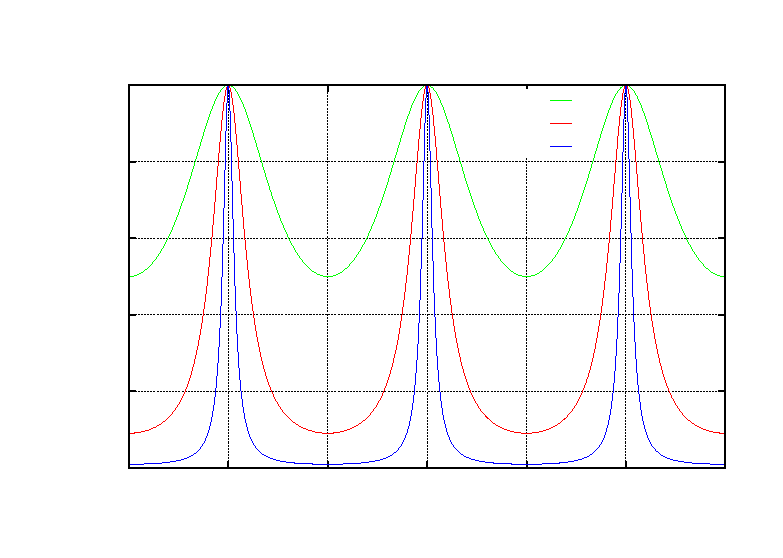
\includegraphics{eps/Airy}}%
    \gplfronttext
  \end{picture}%
\endgroup

\caption{The Airy function peaks when the phase shift is an integer multiple of $2\pi$. As the finesse coefficient increases, the peaks become more sharp and their position is better defined.}
\label{Airyplot}
\end{figure}
\subsection{Interference pattern}
As is clear from \cref{Airyplot}, the interference maxima take place for $\Delta=2m\pi$, where $m$ is an integer representing the order of diffraction.
From \cref{phase} we have
\mate
m=\frac{2n'}{\lambda_0}d\cos\theta'
\label{ordine}
\atem
Looking at \cref{intensity} we define the intensity at the maximum and at the minimum as
\begin{eqnarray}
I_{\mbox{max}}&=&\frac{I_T[\Delta=2m\pi]}{I_{0}}=C_{\mbox{peak}}=\frac{T^2}{(1-R)^2}\\
I_{\mbox{min}}&=&\frac{I_T[\Delta=(2m+1)\pi]}{I_{0}}=\frac{T^2}{(1-R)^2+4R}=\frac{T^2}{(1+R)^2}
\end{eqnarray}
We shall now define a \textit{contrast factor}
\mate
\mathcal{C}\equiv\frac{I_{\mbox{max}}}{I_{\mbox{min}}}=\left(\frac{1+R}{1-R}\right)^2=1+F
\atem
which is also a useful parameter in the characterization of an etalon.

To describe how defined are the peaks, we have to consider their full width at half maximum (FWHM). Thus we observe the points around a maximum whose intensity is $I_{T}=I_{\mbox{max}}/2$. They have a phase shift 
\mate
\Delta=2m\pi\pm\frac{\varepsilon}{2}
\atem

where $\varepsilon$ is now the FWHM expressed as a phase. Putting this into \cref{intensity} we get the identity

$$\frac{1}{2}=\frac{1}{1+F\sin^2\frac{\varepsilon}{4}}\quad;$$ $$F\sin^2\frac{\varepsilon}{4}=1$$

If now we approximate $\sin\frac{\varepsilon}{4}\simeq\frac{\varepsilon}{4}$ we get the phase expression for the FWHM, as a function of the coefficient of finesse $F$
\mate
\varepsilon=\frac{4}{\sqrt{F}}
\atem
Since two contiguous maxima are separated by a phase of $2\pi$, we can do the ratio between the peaks separation and their width, getting a very important parameter which is called the \textit{finesse} of the etalon
\mate
\mathcal{F}\equiv\frac{2\pi}{\varepsilon}=\frac{\pi}{2}\sqrt{F}=\frac{\pi\sqrt{R}}{1-R}
\label{finesse}
\atem
\subsection{Etalon as a spectroscope}
It is possible to build a direct relationship between the angular separation of the rings and the wavelength $\lambda_0$ of the incident light.
We put ourself under the approximation of nearly perpendicular incident light, so that
$$\sin\theta'\simeq\theta'$$$$\sin\theta\simeq\theta$$
Snell's law then simplifies to
$$\frac{\sin\theta'}{n'}=\frac{\sin\theta}{n}\quad\Rightarrow\quad\frac{\theta'}{n'}=\frac{\theta}{n}$$
The small angles approximation also implies
\begin{eqnarray} 
\nonumber\cos\theta'&\simeq&1-\frac{\theta'^2}{2}\\&\simeq&1-\left(\frac{n'}{n}\right)^2\frac{\theta^2}{2}\nonumber
\end{eqnarray}
These approximations being valid, we recall \cref{ordine}
$$m=\frac{2n'}{\lambda_0}d\cos\theta'\quad\Rightarrow\quad m=\frac{2n'}{\lambda_0}d\left(1-\left(\frac{n'}{n}\right)^2\frac{\theta^2}{2}\right)$$
Inverting this one we find
NON SI CAPISCE DA DOVE LA TIRA FUORI E COME, CI SONO CONTI OSCURI [$\dots$]
The angle for the p\textit{th} order is
\mate
\theta_p=\frac{1}{n}\sqrt{\frac{n'\lambda_0}{d}}\sqrt{p-1+e}
\atem
and if we focus the rings onto a screen with a convergent lens, of focal ratio $f$, the diameter of the bright ring is
\mate
D^2_p=(2f\theta_p)^2=\frac{4n'\lambda_0f^2}{n^2d}(p-1+e)
\atem
\end{document}